% answers.tex —— 2022 年·新高考Ⅱ卷 · 参考答案与详细解析片段
% 由 tools/generate_projects.py 依来源总账自 2022/2022_数学真题_新高考Ⅱ_试题.md + 2022/2022_数学真题_新高考Ⅱ_解析正文.md + 2022/2022_数学真题_新高考Ⅱ_答案要点.md 生成，勿手改（改源 MD 后重跑）


\begin{gknotice}
\textbf{解析归属}：试题原文取自 deekur/gaokaomath（commit \texttt{34c13a6}，CC BY 4.0）之 \texttt{2022新高考2} PDF；本文档全部解析由本库编写者根据试题独立推导，\textbf{非官方标准答案}。推导过程完整给出以便核验；若与官方发布版本不一致，以官方为准。
\end{gknotice}

\par\medskip

\gkpart{一、单选题（每小题 5 分，共 40 分）}

\begin{answer}
\gksolhead{1}{}

\textbf{题目}：

已知集合 $A=\{-1,1,2,4\}$，$B=\{x\mid|x-1|\le1\}$，则 $A\cap B=$\mbox{（　　）}

\begin{gkopts}(4)
\task A．$\{-1,2\}$
\task B．$\{1,2\}$
\task C．$\{1,4\}$
\task D．$\{-1,4\}$
\end{gkopts}

\Needspace{4\baselineskip}
\textbf{解析}

\textbf{第一步，把 $B$ 解成区间。}

绝对值不等式 $|x-1|\le1$ 等价于
\nopagebreak[4]
\[-1\le x-1\le1\]

各边加 $1$：
\nopagebreak[4]
\[0\le x\le2\]

即 $B=[0,2]$。

\textbf{第二步，逐个检验 $A$ 中的元素。}

\begin{itemize}
\item $-1\notin[0,2]$（小于 $0$）；
\item $1\in[0,2]$ ；
\item $2\in[0,2]$ （\textbf{端点取得到}，因为是 $\le$）；
\item $4\notin[0,2]$。
\end{itemize}

\nopagebreak[4]
\[A\cap B=\{1,2\}\]

\begin{gktip}
\textbf{易错点}：$2$ 是区间的\textbf{右端点}，$|2-1|=1\le1$ 成立，必须保留。若把 $\le$ 看成 $<$ 就会漏掉 $2$ 而误选 C 或 D 之外的干扰项。含绝对值的集合先化成区间再验元素，比逐个代入更不易出错。
\end{gktip}

\gkanswer{答案：B}

\par\medskip

\end{answer}
\begin{answer}
\gksolhead{2}{}

\textbf{题目}：

$(2+2\mathrm i)(1-2\mathrm i)=$\mbox{（　　）}

\begin{gkopts}(4)
\task A．$-2+4\mathrm i$
\task B．$-2-4\mathrm i$
\task C．$6+2\mathrm i$
\task D．$6-2\mathrm i$
\end{gkopts}

\Needspace{4\baselineskip}
\textbf{解析}

按多项式乘法展开：
\nopagebreak[4]
\[(2+2\mathrm i)(1-2\mathrm i)=2\times1+2\times(-2\mathrm i)+2\mathrm i\times1+2\mathrm i\times(-2\mathrm i)\]

\nopagebreak[4]
\[=2-4\mathrm i+2\mathrm i-4\mathrm i^{2}\]

利用 $\mathrm i^{2}=-1$，末项 $-4\mathrm i^{2}=+4$：
\nopagebreak[4]
\[=(2+4)+(-4+2)\mathrm i=6-2\mathrm i\]

\begin{gktip}
\textbf{速算法}：只看实部就能定答案。实部 $=2\times1-2\times(-2)=2+4=6$，四个选项中实部为 $6$ 的只有 C、D；再看虚部 $=2\times(-2)+2\times1=-2$，锁定 D。复数选择题\textbf{先算一个部分再排除}通常比完整展开更快。
\end{gktip}

\gkanswer{答案：D}

\par\medskip

\end{answer}
\begin{answer}
\gksolhead{3}{}

\textbf{题目}：

图 1 是中国的古建筑中的举架结构，$AA'$，$BB'$，$CC'$，$DD'$ 是桁，相邻桁的水平距离称为步，垂直距离称为举。图 2 是某古建筑屋顶截面示意图，其中 $DD_1$，$CC_1$，$BB_1$，$AA_1$ 是举，$OD_1$，$DC_1$，$CB_1$，$BA_1$ 是相等的步，相邻桁的举步之比分别为 $\dfrac{DD_1}{OD_1}=0.5$，$\dfrac{CC_1}{DC_1}=k_1$，$\dfrac{BB_1}{CB_1}=k_2$，$\dfrac{AA_1}{BA_1}=k_3$。已知 $k_1$，$k_2$，$k_3$ 成公差为 $0.1$ 的等差数列，且直线 $OA$ 的斜率为 $0.725$，则 $k_3=$\mbox{（　　）}
\nopagebreak[4]
\begin{center}% 2022 新高考Ⅱ卷 3：中国古建筑「举架」结构（简化示意图）
% 原图为木构屋架写实线描，此处按简化示意重绘，不追求写实细节，只保留题意所需的阶梯关系：
% 底部大梁之上叠三层逐层收短的横梁，层间以瓜柱（短柱）支撑，梁端置桁（檩）。
% 相邻桁的水平距离（步）恒取 1，瓜柱高（举）自下而上取 0.5、0.7、0.8、0.9，
% 故屋面折线呈上陡下缓。右半侧自上而下标桁位 A'、B'、C'、D'，其正下方梁上对应点标 A、B、C、D，
% 竖直段 AA'、BB'、CC'、DD' 即「举」，相邻两点的水平间距即「步」。
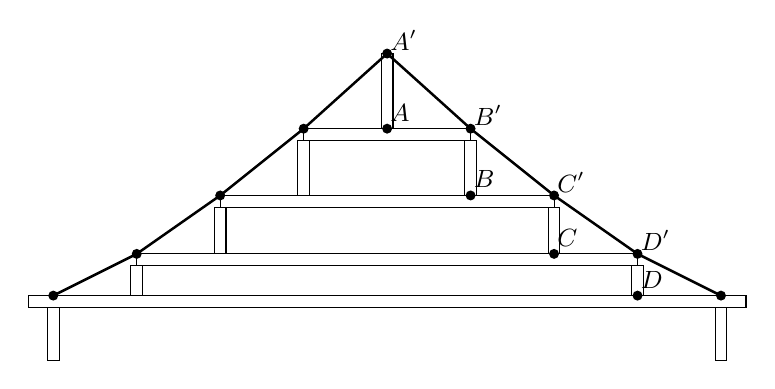
\begin{tikzpicture}[scale=1.06, font=\small]
  % ---- 梁：自下而上逐层收短（细长矩形示木料截面）----
  \draw (-4.3,-0.14) rectangle (4.3,0);
  \draw (-3,0.36)    rectangle (3,0.5);
  \draw (-2,1.06)    rectangle (2,1.2);
  \draw (-1,1.86)    rectangle (1,2.0);
  % ---- 檐柱（示意落地）----
  \draw (-4.07,-0.78) rectangle (-3.93,-0.14);
  \draw (3.93,-0.78)  rectangle (4.07,-0.14);
  % ---- 瓜柱：层间短柱，其高即「举」----
  \foreach \s in {-1,1}{
    \draw (3*\s-0.07,0)   rectangle (3*\s+0.07,0.36);
    \draw (2*\s-0.07,0.5) rectangle (2*\s+0.07,1.06);
    \draw (\s-0.07,1.2)   rectangle (\s+0.07,1.86);
  }
  \draw (-0.07,2.0) rectangle (0.07,2.9);          % 脊瓜柱
  % ---- 屋面折线：依次过各桁位 ----
  \draw[line width=0.9pt]
    (-4,0) -- (-3,0.5) -- (-2,1.2) -- (-1,2.0) -- (0,2.9)
           -- (1,2.0) -- (2,1.2) -- (3,0.5) -- (4,0);
  % ---- 桁位标记 ----
  \foreach \p in {(-4,0),(-3,0.5),(-2,1.2),(-1,2.0),(0,2.9),(1,2.0),(2,1.2),(3,0.5),(4,0)}
    { \fill \p circle (1.7pt); }
  \foreach \p in {(0,2.0),(1,1.2),(2,0.5),(3,0)} { \fill \p circle (1.7pt); }
  % ---- 标注（右半侧）----
  \node[above right, inner sep=1pt] at (0,2.9) {$A'$};
  \node[above right, inner sep=1pt] at (1,2.0) {$B'$};
  \node[above right, inner sep=1pt] at (2,1.2) {$C'$};
  \node[above right, inner sep=1pt] at (3,0.5) {$D'$};
  \node[above right, inner sep=1pt, yshift=1.5pt] at (0,2.0) {$A$};
  \node[above right, inner sep=1pt, yshift=1.5pt] at (1,1.2) {$B$};
  \node[above right, inner sep=1pt, yshift=1.5pt] at (2,0.5) {$C$};
  \node[above right, inner sep=1pt, yshift=1.5pt] at (3,0)   {$D$};
\end{tikzpicture}
\end{center}
\nopagebreak[4]
\nopagebreak[4]
\begin{center}% 2022 新高考Ⅱ卷 3：举架结构抽象出的屋顶截面折线图
% 左半支自原点 O 经 D、C、B 升至顶点 A，右半支关于过 A 的竖直线对称（不标字母）。
% 步长恒为 1，举依次取 0.5、0.7、0.8、0.9，即 O(0,0)、D(1,0.5)、C(2,1.2)、B(3,2.0)、A(4,2.9)。
% 虚线小阶梯给出各段的举与步：垂足 D_1(1,0)、C_1(2,0.5)、B_1(3,1.2)、A_1(4,2.0)，
% 水平段 OD_1、DC_1、CB_1、BA_1 四段等长（即「步」），竖直段 DD_1、CC_1、BB_1、AA_1 即「举」。
\begin{tikzpicture}[scale=1.12, font=\small]
  % ---- 坐标轴 ----
  \draw[-stealth] (-0.45,0) -- (8.95,0);
  \draw[-stealth] (0,-0.4) -- (0,3.45);
  % ---- 举步阶梯（虚线）----
  \draw[dashed] (0,0) -- (1,0) -- (1,0.5) -- (2,0.5) -- (2,1.2)
                     -- (3,1.2) -- (3,2.0) -- (4,2.0) -- (4,2.9);
  % ---- 屋顶截面折线 ----
  \draw[line width=0.9pt]
    (0,0) -- (1,0.5) -- (2,1.2) -- (3,2.0) -- (4,2.9)
          -- (5,2.0) -- (6,1.2) -- (7,0.5) -- (8,0);
  % ---- 点 ----
  \foreach \p in {(0,0),(1,0.5),(2,1.2),(3,2.0),(4,2.9),(1,0),(2,0.5),(3,1.2),(4,2.0)}
    { \fill \p circle (1.6pt); }
  % ---- 标注：折线点在左上，垂足在下/右 ----
  \node[below left,  inner sep=2pt] at (0,0)   {$O$};
  \node[above left,  inner sep=1pt] at (1,0.5) {$D$};
  \node[above left,  inner sep=1pt] at (2,1.2) {$C$};
  \node[above left,  inner sep=1pt] at (3,2.0) {$B$};
  \node[above,       inner sep=2pt] at (4,2.9) {$A$};
  \node[below,       inner sep=2pt] at (1,0)   {$D_1$};
  \node[below right, inner sep=1pt] at (2,0.5) {$C_1$};
  \node[below right, inner sep=1pt] at (3,1.2) {$B_1$};
  \node[below right, inner sep=1pt] at (4,2.0) {$A_1$};
\end{tikzpicture}
\end{center}
\nopagebreak[4]
\begin{gkopts}(4)
\task A．$0.75$
\task B．$0.8$
\task C．$0.85$
\task D．$0.9$
\end{gkopts}

\Needspace{4\baselineskip}
\textbf{解析}

\textbf{第一步，把"步相等"这个条件用上。}

四个步 $OD_1$、$DC_1$、$CB_1$、$BA_1$ 长度相等，\textbf{不妨设每步长为 $1$}（斜率是比值，与单位无关）。

于是四个举（竖直上升量）依次为
\nopagebreak[4]
\[DD_1=0.5,\qquad CC_1=k_1,\qquad BB_1=k_2,\qquad AA_1=k_3\]

\textbf{第二步，把斜率写成"总举 ÷ 总步"。}

从 $O$ 到 $A$，水平方向累计走了 $4$ 个步，竖直方向累计上升了四个举之和：
\nopagebreak[4]
\[k_{OA}=\frac{0.5+k_1+k_2+k_3}{4}=0.725\]

\nopagebreak[4]
\[0.5+k_1+k_2+k_3=2.9\ \Longrightarrow\ k_1+k_2+k_3=2.4\]

\textbf{第三步，用等差数列的对称性。}

$k_1$，$k_2$，$k_3$ 成等差，中间项 $k_2$ 是三者的平均数：
\nopagebreak[4]
\[k_2=\frac{k_1+k_2+k_3}3=\frac{2.4}3=0.8\]

公差为 $0.1$：
\nopagebreak[4]
\[k_3=k_2+0.1=0.9\]

\textbf{验证}：$k_1=0.7$、$k_2=0.8$、$k_3=0.9$，总举 $=0.5+0.7+0.8+0.9=2.9$，$\dfrac{2.9}4=0.725$ 

\begin{gktip}
\textbf{建模要点}：本题的全部难度在于读懂"直线 $OA$ 的斜率"指的是\textbf{从起点到终点的整体斜率}，而不是某一段的斜率——即 $k_{OA}=\dfrac{\text{\text{各举之和}}}{\text{\text{各步之和}}}$。中国古建筑的举架正是靠\textbf{逐段增大举步比}做出屋面的反曲线，各段斜率递增而整体斜率取平均，这也是"$k_2$ 恰为三数平均"这一巧解的物理来源。
\end{gktip}

\gkanswer{答案：D（$0.9$）}

\par\medskip

\end{answer}
\begin{answer}
\gksolhead{4}{}

\textbf{题目}：

已知向量 $\boldsymbol a=(3,4)$，$\boldsymbol b=(1,0)$，$\boldsymbol c=\boldsymbol a+t\boldsymbol b$，若 $\langle\boldsymbol a,\boldsymbol c\rangle=\langle\boldsymbol b,\boldsymbol c\rangle$，则 $t=$\mbox{（　　）}

\begin{gkopts}(4)
\task A．$-6$
\task B．$-5$
\task C．$5$
\task D．$6$
\end{gkopts}

\Needspace{4\baselineskip}
\textbf{解析}

\textbf{第一步，写出 $\boldsymbol c$。}
\nopagebreak[4]
\[\boldsymbol c=\boldsymbol a+t\boldsymbol b=(3+t,\ 4)\]

\textbf{第二步，把"两个夹角相等"翻译成方程。}

夹角相等等价于余弦相等：
\nopagebreak[4]
\[\frac{\boldsymbol a\cdot\boldsymbol c}{|\boldsymbol a||\boldsymbol c|}=\frac{\boldsymbol b\cdot\boldsymbol c}{|\boldsymbol b||\boldsymbol c|}\]

两边同乘 $|\boldsymbol c|$（$\boldsymbol c\ne\boldsymbol0$，因为第二个分量恒为 $4$），\textbf{公共因子 $|\boldsymbol c|$ 直接消掉}：
\nopagebreak[4]
\[\frac{\boldsymbol a\cdot\boldsymbol c}{|\boldsymbol a|}=\frac{\boldsymbol b\cdot\boldsymbol c}{|\boldsymbol b|}\]

\textbf{第三步，代入数据。}
\nopagebreak[4]
\[\boldsymbol a\cdot\boldsymbol c=3(3+t)+4\times4=25+3t,\qquad|\boldsymbol a|=\sqrt{9+16}=5\]
\nopagebreak[4]
\[\boldsymbol b\cdot\boldsymbol c=1\times(3+t)+0\times4=3+t,\qquad|\boldsymbol b|=1\]

\nopagebreak[4]
\[\frac{25+3t}5=3+t\]

\nopagebreak[4]
\[25+3t=15+5t\ \Longrightarrow\ 2t=10\ \Longrightarrow\ t=5\]

\textbf{验证}（$t=5$ 时 $\boldsymbol c=(8,4)$）：
\nopagebreak[4]
\[\cos\langle\boldsymbol a,\boldsymbol c\rangle=\frac{24+16}{5\times\sqrt{80}}=\frac{40}{5\times4\sqrt5}=\frac{2}{\sqrt5},\qquad\cos\langle\boldsymbol b,\boldsymbol c\rangle=\frac{8}{1\times4\sqrt5}=\frac2{\sqrt5}\]
两者相等 

\begin{gktip}
\textbf{关键技巧}：夹角相等的条件里，$|\boldsymbol c|$ 是两边共有的，\textbf{先约掉再代数}能把一个含根号的方程降为一次方程。若硬着头皮平方展开，会得到一个可解但繁琐的二次方程，还要额外验根（平方会引入 $\cos$ 相反的假根）。

\textbf{几何解读}：$\boldsymbol c$ 与 $\boldsymbol a$、$\boldsymbol b$ 夹角相等，说明 $\boldsymbol c$ 落在 $\boldsymbol a$、$\boldsymbol b$ 张成的角的\textbf{平分线方向}上，即 $\boldsymbol c\parallel\dfrac{\boldsymbol a}{|\boldsymbol a|}+\dfrac{\boldsymbol b}{|\boldsymbol b|}=\left(\dfrac35+1,\dfrac45\right)=\left(\dfrac85,\dfrac45\right)\parallel(2,1)$。由 $(3+t,4)\parallel(2,1)$ 得 $3+t=8$，$t=5$，这是最快的一条路。
\end{gktip}

\gkanswer{答案：C（$5$）}

\par\medskip

\end{answer}
\begin{answer}
\gksolhead{5}{}

\textbf{题目}：

甲、乙、丙、丁、戊 $5$ 名同学站成一排参加文艺汇演，若甲不站在两端，丙和丁相邻，则不同排列方式共有\mbox{（　　）}

\begin{gkopts}(4)
\task A．$12$ 种
\task B．$24$ 种
\task C．$36$ 种
\task D．$48$ 种
\end{gkopts}

\Needspace{4\baselineskip}
\textbf{解析}

\textbf{第一步，用捆绑法处理"丙丁相邻"。}

把丙、丁看成一个整体（记作 $\square$），则要排列的对象为：甲、乙、戊、$\square$，共 $4$ 个。$4$ 个对象全排列 $A_4^4=24$ 种，$\square$ 内部丙丁可交换，乘 $2$：
\nopagebreak[4]
\[\text{\text{丙丁相邻的总排法}}=A_4^4\times A_2^2=24\times2=48\]

\textbf{第二步，用"正难则反"减去甲在两端的情形。}

注意 $\square$ 占据原来 $5$ 个座位中相邻的两个，所以\textbf{不能}直接说"甲在 $4$ 个对象里占 $2$ 个端点位置"——必须回到 $5$ 个座位来数。

\textbf{甲站第 $1$ 位}：剩余座位 $2,3,4,5$ 分给乙、戊、$\square$。$\square$ 需要相邻两个座位，可选 $(2,3)$、$(3,4)$、$(4,5)$ 共 $3$ 种；$\square$ 内部 $2$ 种；剩下 $2$ 个座位排乙、戊有 $A_2^2=2$ 种：
\nopagebreak[4]
\[3\times2\times2=12\]

\textbf{甲站第 $5$ 位}：由对称性同样是 $12$ 种。

\nopagebreak[4]
\[\text{\text{甲在两端的排法}}=12+12=24\]

\textbf{第三步，作差。}
\nopagebreak[4]
\[48-24=24\]

\textbf{枚举验证}：用程序穷举 $5!=120$ 种排列，筛选出"甲不在首尾且丙丁相邻"的，恰得 $24$ 种 

\begin{gktip}
\textbf{陷阱说明}：捆绑后对象只剩 $4$ 个，很容易顺手写成"甲在两端 $=2\times A_3^3\times A_2^2=24$"——这个式子把 $\square$ 当成一个普通座位，\textbf{算的是"甲在 $4$ 个对象序列的两端"}，与"甲在 $5$ 个座位的两端"恰好数值相同（都是 $24$），纯属巧合。一旦题目改成"甲不站在第 $2$ 位"，两种口径就会分家。\textbf{捆绑法之后，凡涉及"具体位置"的限制，一律回到原座位数}。

\textbf{另解（插空法）}：先排乙、戊得 $A_2^2=2$ 种，产生 $3$ 个空位……本题因"甲不在两端"与"丙丁相邻"两个限制交织，直接分类反而不如上面的补集法干净。
\end{gktip}

\gkanswer{答案：B（$24$ 种）}

\par\medskip

\end{answer}
\begin{answer}
\gksolhead{6}{}

\textbf{题目}：

若 $\sin(\alpha+\beta)+\cos(\alpha+\beta)=2\sqrt2\cos\left(\alpha+\dfrac\pi4\right)\sin\beta$，则\mbox{（　　）}

\begin{gkopts}(2)
\task A．$\tan(\alpha-\beta)=1$
\task B．$\tan(\alpha+\beta)=1$
\task C．$\tan(\alpha-\beta)=-1$
\task D．$\tan(\alpha+\beta)=-1$
\end{gkopts}

\Needspace{4\baselineskip}
\textbf{解析}

\textbf{第一步，把右边的 $\sqrt2\cos\left(\alpha+\dfrac\pi4\right)$ 拆开。}
\nopagebreak[4]
\[\sqrt2\cos\left(\alpha+\frac\pi4\right)=\sqrt2\left(\cos\alpha\cos\frac\pi4-\sin\alpha\sin\frac\pi4\right)=\cos\alpha-\sin\alpha\]

于是
\nopagebreak[4]
\[\text{\text{右边}}=2(\cos\alpha-\sin\alpha)\sin\beta=2\sin\beta\cos\alpha-2\sin\alpha\sin\beta\]

\textbf{第二步，把左边按和角公式展开。}
\nopagebreak[4]
\[\sin(\alpha+\beta)=\sin\alpha\cos\beta+\cos\alpha\sin\beta\]
\nopagebreak[4]
\[\cos(\alpha+\beta)=\cos\alpha\cos\beta-\sin\alpha\sin\beta\]

\nopagebreak[4]
\[\text{\text{左边}}=\sin\alpha\cos\beta+\cos\alpha\sin\beta+\cos\alpha\cos\beta-\sin\alpha\sin\beta\]

\textbf{第三步，移项合并。}

左边减右边：
\nopagebreak[4]
\[\sin\alpha\cos\beta+\cos\alpha\sin\beta+\cos\alpha\cos\beta-\sin\alpha\sin\beta-2\cos\alpha\sin\beta+2\sin\alpha\sin\beta=0\]

逐项合并：

\begin{itemize}
\item $\cos\alpha\sin\beta-2\cos\alpha\sin\beta=-\cos\alpha\sin\beta$；
\item $-\sin\alpha\sin\beta+2\sin\alpha\sin\beta=+\sin\alpha\sin\beta$。
\end{itemize}

\nopagebreak[4]
\[\underbrace{\sin\alpha\cos\beta-\cos\alpha\sin\beta}_{\sin(\alpha-\beta)}+\underbrace{\cos\alpha\cos\beta+\sin\alpha\sin\beta}_{\cos(\alpha-\beta)}=0\]

\textbf{第四步，得出结论。}
\nopagebreak[4]
\[\sin(\alpha-\beta)+\cos(\alpha-\beta)=0\]

因为 $\cos(\alpha-\beta)=0$ 时上式给出 $\sin(\alpha-\beta)=0$，与 $\sin^2+\cos^2=1$ 矛盾，故 $\cos(\alpha-\beta)\ne0$，两边同除：
\nopagebreak[4]
\[\tan(\alpha-\beta)=-1\]

\textbf{数值验证}：随机取 $\alpha$，数值求解原方程得到的 $\beta$，代入四个选项检验——$2261$ 组解中 $\tan(\alpha-\beta)=-1$ 全部成立，其余三项\textbf{一次都没成立} 

\begin{gktip}
\textbf{方法总结}：题目里出现 $\cos\left(\alpha+\dfrac\pi4\right)$ 且系数带 $\sqrt2$，\textbf{这是"辅助角公式的逆用"信号}——$\sqrt2\cos\left(\alpha+\dfrac\pi4\right)=\cos\alpha-\sin\alpha$，先把它化掉，整个式子就变成纯粹的展开与合并。四个选项分别对应 $\alpha\pm\beta$ 的正切等于 $\pm1$，暗示最终一定会凑出 $\sin(\alpha\pm\beta)\pm\cos(\alpha\pm\beta)=0$ 的形式，\textbf{合并时要有意识地朝 $\alpha-\beta$ 的和差公式凑}。
\end{gktip}

\gkanswer{答案：C（$\tan(\alpha-\beta)=-1$）}

\par\medskip

\end{answer}
\begin{answer}
\gksolhead{7}{}

\textbf{题目}：

已知正三棱台的高为 $1$，上、下底面的边长分别为 $3\sqrt3$ 和 $4\sqrt3$，其顶点都在同一球面上，则该球的表面积为\mbox{（　　）}

\begin{gkopts}(4)
\task A．$100\pi$
\task B．$128\pi$
\task C．$144\pi$
\task D．$192\pi$
\end{gkopts}

\Needspace{4\baselineskip}
\textbf{解析}

\textbf{第一步，求两个底面的外接圆半径。}

正三角形边长 $s$ 时，外接圆半径 $r=\dfrac s{\sqrt3}$（由正弦定理 $\dfrac s{\sin60^\circ}=2r$ 得 $r=\dfrac s{\sqrt3}$）。

\begin{itemize}
\item 上底面：$s_1=3\sqrt3\Rightarrow r_1=\dfrac{3\sqrt3}{\sqrt3}=3$
\item 下底面：$s_2=4\sqrt3\Rightarrow r_2=\dfrac{4\sqrt3}{\sqrt3}=4$
\end{itemize}

\textbf{第二步，建立轴向坐标。}

棱台的两个底面平行，六个顶点都在球面上 $\Rightarrow$ 球心必在\textbf{两底面中心的连线（棱台的轴）}上。

以下底面中心为原点，轴为 $z$ 轴，则下底面在 $z=0$、上底面在 $z=1$（高为 $1$）。设球心为 $(0,0,t)$，半径 $R$。

\textbf{第三步，对两个底面各写一次勾股关系。}

球心到下底面顶点：
\nopagebreak[4]
\[R^{2}=r_2^{2}+t^{2}=16+t^{2}\]

球心到上底面顶点：
\nopagebreak[4]
\[R^{2}=r_1^{2}+(t-1)^{2}=9+(t-1)^{2}\]

\textbf{第四步，解出 $t$ 与 $R$。}
\nopagebreak[4]
\[16+t^{2}=9+t^{2}-2t+1\]
\nopagebreak[4]
\[16=10-2t\ \Longrightarrow\ t=-3\]

\nopagebreak[4]
\[R^{2}=16+(-3)^{2}=25\ \Longrightarrow\ R=5\]

\textbf{第五步，求表面积。}
\nopagebreak[4]
\[S=4\pi R^{2}=4\pi\times25=100\pi\]

\begin{gktip}
\textbf{结论的几何含义}：$t=-3<0$ 说明\textbf{球心并不在棱台内部，而在下底面之下 $3$ 个单位处}。很多同学默认球心夹在两底面之间，于是设两段距离为 $d$ 与 $1-d$，解出 $d=-3$ 后以为算错而反复重算。

\textbf{规避办法}：用\textbf{带符号的坐标 $t$}（而不是"距离 $d$"）建立方程，解出负值只表示方向，不表示矛盾。这是一切"多面体外接球"问题的通用设法。

\textbf{反向验算}：$R=5$，球心 $(0,0,-3)$。下底面顶点到球心距离 $=\sqrt{16+9}=5$ ；上底面顶点到球心距离 $=\sqrt{9+16}=5$ （$t-1=-4$）。
\end{gktip}

\gkanswer{答案：A（$100\pi$）}

\par\medskip

\end{answer}
\begin{answer}
\gksolhead{8}{}

\textbf{题目}：

已知函数 $f(x)$ 的定义域为 $\mathbf R$，且 $f(x+y)+f(x-y)=f(x)f(y)$，$f(1)=1$，则 $\displaystyle\sum_{k=1}^{22}f(k)=$\mbox{（　　）}

\begin{gkopts}(4)
\task A．$-3$
\task B．$-2$
\task C．$0$
\task D．$1$
\end{gkopts}

\Needspace{4\baselineskip}
\textbf{解析}

\textbf{第一步，先取特殊值求 $f(0)$。}

令 $x=1$，$y=0$：
\nopagebreak[4]
\[f(1)+f(1)=f(1)f(0)\ \Longrightarrow\ 2=f(0)\]

（这里用了 $f(1)=1\ne0$，可以两边约去。）

\textbf{第二步，令 $y=1$ 得到递推。}

在原式中取 $y=1$：
\nopagebreak[4]
\[f(x+1)+f(x-1)=f(x)f(1)=f(x)\]

即
\nopagebreak[4]
\[f(x+1)=f(x)-f(x-1)\qquad(\ast)\]

\textbf{第三步，用 $(\ast)$ 逐个算出整数值。}

已知 $f(0)=2$，$f(1)=1$：

\begin{center}
\begingroup\setlength{\tabcolsep}{4pt}
\begin{tabular}{ccccccccc}
\toprule
$k$ & $0$ & $1$ & $2$ & $3$ & $4$ & $5$ & $6$ & $7$ \\
\midrule
$f(k)$ & $2$ & $1$ & $-1$ & $-2$ & $-1$ & $1$ & $2$ & $1$ \\
\bottomrule
\end{tabular}
\endgroup
\end{center}

逐步：$f(2)=f(1)-f(0)=1-2=-1$；$f(3)=f(2)-f(1)=-1-1=-2$；$f(4)=f(3)-f(2)=-2+1=-1$；$f(5)=f(4)-f(3)=-1+2=1$；$f(6)=f(5)-f(4)=1+1=2$；$f(7)=f(6)-f(5)=2-1=1$。

\textbf{第四步，识别周期。}

$f(6)=f(0)$ 且 $f(7)=f(1)$，而递推 $(\ast)$ 只依赖前两项，故
\nopagebreak[4]
\[f(k+6)=f(k)\]

\textbf{周期为 $6$}。（也可由 $(\ast)$ 直接推：$f(x+3)=f(x+2)-f(x+1)=\left[f(x+1)-f(x)\right]-f(x+1)=-f(x)$，故 $f(x+6)=-f(x+3)=f(x)$。）

\textbf{第五步，分组求和。}

一个完整周期的和：
\nopagebreak[4]
\[f(1)+f(2)+\cdots+f(6)=1-1-2-1+1+2=0\]

$22=3\times6+4$，前 $18$ 项恰好三个完整周期，和为 $0$：
\nopagebreak[4]
\[\sum_{k=1}^{22}f(k)=0+f(19)+f(20)+f(21)+f(22)=f(1)+f(2)+f(3)+f(4)=1-1-2-1=-3\]

\textbf{独立验证（找出一个具体的 $f$）}：取 $f(x)=2\cos\dfrac{\pi x}3$。由和差化积
\nopagebreak[4]
\[f(x+y)+f(x-y)=2\left[\cos\frac{\pi(x+y)}3+\cos\frac{\pi(x-y)}3\right]=4\cos\frac{\pi x}3\cos\frac{\pi y}3=f(x)f(y)\]
且 $f(1)=2\cos\dfrac\pi3=1$  满足全部条件。程序在 $625$ 组 $(x,y)$ 上核验函数方程全部成立，且 $\displaystyle\sum_{k=1}^{22}f(k)=-3$ 

\begin{gktip}
\textbf{方法总结}：抽象函数题的标准三步是"\textbf{赋特殊值 → 造递推 → 找周期}"。本题的关键赋值有两个：$y=0$ 定出 $f(0)=2$（缺了它递推无法启动），$y=1$ 把二元函数方程降为一元递推。

\textbf{提速技巧}：$f(x+3)=-f(x)$ 这个"半周期反号"的性质比周期 $6$ 更好用——它直接说明\textbf{任意连续 $6$ 项之和为 $0$}，于是 $22$ 项只需算余下的 $4$ 项。

\textbf{反例警戒}：不要以为满足 $f(x+y)+f(x-y)=f(x)f(y)$ 的函数只有余弦型。该方程（达朗贝尔方程）在不加连续性假设时还有病态解，但本题只问整数点的值，由递推唯一确定，与是否连续无关。
\end{gktip}

\gkanswer{答案：A（$-3$）}

\par\medskip

\end{answer}
\gkpart{二、多选题（每小题 5 分，共 20 分）}

\begin{answer}
\gksolhead{9}{}

\textbf{题目}：

已知函数 $f(x)=\sin(2x+\varphi)\ (0<\varphi<\pi)$ 的图象关于点 $\left(\dfrac{2\pi}3,0\right)$ 中心对称，则\mbox{（　　）}

\begin{gkopts}(1)
\task A．$f(x)$ 在区间 $\left(0,\dfrac{5\pi}{12}\right)$ 单调递减
\task B．$f(x)$ 在区间 $\left(-\dfrac\pi{12},\dfrac{11\pi}{12}\right)$ 有两个极值点
\task C．直线 $x=\dfrac{7\pi}6$ 是曲线 $y=f(x)$ 的对称轴
\task D．直线 $y=\dfrac{\sqrt3}2-x$ 是曲线 $y=f(x)$ 的切线
\end{gkopts}

\Needspace{4\baselineskip}
\textbf{解析}

\textbf{预备：先定出 $\varphi$。}

正弦曲线的对称中心就是它的零点，故
\nopagebreak[4]
\[\sin\left(2\times\frac{2\pi}3+\varphi\right)=0\ \Longrightarrow\ \frac{4\pi}3+\varphi=k\pi\ (k\in\mathbf Z)\]

\nopagebreak[4]
\[\varphi=k\pi-\frac{4\pi}3\]

代入 $0<\varphi<\pi$：$k=2$ 时 $\varphi=2\pi-\dfrac{4\pi}3=\dfrac{2\pi}3$（$k=1$ 给 $-\dfrac\pi3<0$，$k=3$ 给 $\dfrac{5\pi}3>\pi$，都不合）。

\nopagebreak[4]
\[\boxed{f(x)=\sin\left(2x+\frac{2\pi}3\right)},\qquad f'(x)=2\cos\left(2x+\frac{2\pi}3\right)\]

以下把 $u=2x+\dfrac{2\pi}3$ 称为\textbf{相位}，四个选项都通过相位的取值范围判断。

\par\medskip

\textbf{A 项}：$x\in\left(0,\dfrac{5\pi}{12}\right)$ 时
\nopagebreak[4]
\[u\in\left(\frac{2\pi}3,\ \frac{5\pi}6+\frac{2\pi}3\right)=\left(\frac{2\pi}3,\ \frac{3\pi}2\right)\]

$\sin u$ 在 $\left[\dfrac\pi2,\dfrac{3\pi}2\right]$ 上单调递减，而 $\dfrac{2\pi}3>\dfrac\pi2$，所以区间 $\left(\dfrac{2\pi}3,\dfrac{3\pi}2\right)$ \textbf{完全落在递减段内}  \textbf{正确}。

（程序在该区间取 $2$ 万个点，$f'(x)<0$ 全部成立 ）

\par\medskip

\textbf{B 项}：$x\in\left(-\dfrac\pi{12},\dfrac{11\pi}{12}\right)$ 时
\nopagebreak[4]
\[u\in\left(-\frac\pi6+\frac{2\pi}3,\ \frac{11\pi}6+\frac{2\pi}3\right)=\left(\frac\pi2,\ \frac{5\pi}2\right)\]

极值点对应 $\cos u=0$，即 $u=\dfrac\pi2+k\pi$。在\textbf{开区间} $\left(\dfrac\pi2,\dfrac{5\pi}2\right)$ 内，$\dfrac\pi2$ 与 $\dfrac{5\pi}2$ 都是端点（取不到），只剩 $u=\dfrac{3\pi}2$ 一个。

故只有 \textbf{$1$ 个}极值点  \textbf{错误}。（程序数 $f'$ 的变号次数：$1$ 次  与结论一致。）

\par\medskip

\textbf{C 项}：把 $x=\dfrac{7\pi}6$ 代入相位：
\nopagebreak[4]
\[u=\frac{7\pi}3+\frac{2\pi}3=3\pi\]

对称轴要求 $\sin u=\pm1$，即 $u=\dfrac\pi2+k\pi$；而 $u=3\pi$ 给出 $f\left(\dfrac{7\pi}6\right)=\sin3\pi=0$。

所以 $x=\dfrac{7\pi}6$ 处是\textbf{零点}，对应的是对称\textbf{中心} $\left(\dfrac{7\pi}6,0\right)$，不是对称轴  \textbf{错误}。

\par\medskip

\textbf{D 项}：直线 $y=\dfrac{\sqrt3}2-x$ 的斜率为 $-1$。切点处需
\nopagebreak[4]
\[f'(x)=2\cos u=-1\ \Longrightarrow\ \cos u=-\frac12\ \Longrightarrow\ u=\frac{2\pi}3+2k\pi\ \text{\text{或}}\ u=\frac{4\pi}3+2k\pi\]

\begin{itemize}
\item \textbf{第一支}：$2x+\dfrac{2\pi}3=\dfrac{2\pi}3+2k\pi\Rightarrow x=k\pi$。取 $k=0$：切点 $\left(0,\ \sin\dfrac{2\pi}3\right)=\left(0,\dfrac{\sqrt3}2\right)$，切线为
\end{itemize}
\nopagebreak[4]
\[y-\frac{\sqrt3}2=-(x-0)\ \Longrightarrow\ y=\frac{\sqrt3}2-x\]
  \textbf{正是题目给的直线} 

\begin{itemize}
\item （第二支 $x=\dfrac\pi3+k\pi$ 处切点纵坐标为 $-\dfrac{\sqrt3}2$，切线为 $y=-x+\dfrac\pi3+k\pi-\dfrac{\sqrt3}2$，纵截距对任何整数 $k$ 都不等于 $\dfrac{\sqrt3}2$，与本题无关。）
\end{itemize}

 \textbf{正确}。（程序核验：$f(0)=\dfrac{\sqrt3}2$、$f'(0)=-1$，切点与斜率双双吻合 ）

\begin{gktip}
\textbf{方法总结}：$y=A\sin(\omega x+\varphi)$ 的一切性质题，都可以统一化成"\textbf{相位 $u$ 落在哪个区间}"：
\begin{itemize}
\item 单调递减 $\Leftrightarrow u$ 落在 $\left[\dfrac\pi2+2k\pi,\dfrac{3\pi}2+2k\pi\right]$ 内；
\item 极值点 $\Leftrightarrow u=\dfrac\pi2+k\pi$；
\item 对称轴 $\Leftrightarrow u=\dfrac\pi2+k\pi$；对称中心 $\Leftrightarrow u=k\pi$。
\end{itemize}

\textbf{B 项的开闭之争是本题唯一的坑}：区间端点是否算极值点，取决于区间是开是闭——题目给的是开区间，端点 $u=\dfrac\pi2$ 与 $u=\dfrac{5\pi}2$ 都不算，答案由"两个"变成"一个"。\textbf{算相位区间时务必抄准开闭符号}。
\end{gktip}

\gkanswer{答案：AD}

\par\medskip

\end{answer}
\begin{answer}
\gksolhead{10}{}

\textbf{题目}：

已知 $O$ 为坐标原点，过抛物线 $C:y^{2}=2px\ (p>0)$ 焦点 $F$ 的直线与 $C$ 交于 $A$，$B$ 两点，其中 $A$ 在第一象限，点 $M(p,0)$。若 $|AF|=|AM|$，则\mbox{（　　）}

\begin{gkopts}(2)
\task A．直线 $AB$ 的斜率为 $2\sqrt6$
\task B．$|OB|=|OF|$
\task C．$|AB|>4|OF|$
\task D．$\angle OAM+\angle OBM<180^\circ$
\end{gkopts}

\Needspace{4\baselineskip}
\textbf{解析}

\textbf{预备一：整个图形关于 $p$ 是相似的。}

作位似变换 $(x,y)\mapsto\left(\dfrac xp,\dfrac yp\right)$，抛物线 $y^{2}=2px$ 变为 $y^{2}=2x$，$F$、$M$ 也随之变换。\textbf{长度之比与角度都不变}，因此四个选项的真假与 $p$ 无关。以下取 $p=1$ 计算：
\nopagebreak[4]
\[C:y^{2}=2x,\qquad F\left(\frac12,0\right),\qquad M(1,0),\qquad|OF|=\frac12\]

\textbf{预备二：定出 $A$。}

$|AF|=|AM|$ 说明 $A$ 在线段 $FM$ 的\textbf{垂直平分线}上，故
\nopagebreak[4]
\[x_A=\frac{\frac12+1}2=\frac34\]

代入抛物线（$A$ 在第一象限取正根）：
\nopagebreak[4]
\[y_A^{2}=2\times\frac34=\frac32\ \Longrightarrow\ y_A=\frac{\sqrt6}2\]

\nopagebreak[4]
\[A\left(\frac34,\ \frac{\sqrt6}2\right)\]

\textbf{预备三：定出 $B$。}

设直线 $AB$：$x=my+\dfrac12$，代入 $y^{2}=2x$ 得 $y^{2}-2my-1=0$，由韦达定理
\nopagebreak[4]
\[y_Ay_B=-1\ \Longrightarrow\ y_B=-\frac1{y_A}=-\frac2{\sqrt6}=-\frac{\sqrt6}3\]

\nopagebreak[4]
\[x_B=\frac{y_B^{2}}2=\frac{\frac69}2=\frac13,\qquad B\left(\frac13,\ -\frac{\sqrt6}3\right)\]

\par\medskip

\textbf{A 项}：直线 $AB$ 过 $F$，斜率
\nopagebreak[4]
\[k=\frac{y_A-0}{x_A-\frac12}=\frac{\frac{\sqrt6}2}{\frac34-\frac12}=\frac{\frac{\sqrt6}2}{\frac14}=2\sqrt6\]

 \textbf{正确}。

\par\medskip

\textbf{B 项}：
\nopagebreak[4]
\[|OB|=\sqrt{x_B^{2}+y_B^{2}}=\sqrt{\frac19+\frac69}=\frac{\sqrt7}3\approx0.882\]

而 $|OF|=\dfrac12=0.5$，两者不等  \textbf{错误}。

\par\medskip

\textbf{C 项}：用焦点弦公式 $|AB|=x_A+x_B+p$（两条焦半径分别等于点到准线的距离）：
\nopagebreak[4]
\[|AB|=\frac34+\frac13+1=\frac{9+4+12}{12}=\frac{25}{12}\]

\nopagebreak[4]
\[4|OF|=4\times\frac12=2=\frac{24}{12}\]

\nopagebreak[4]
\[\frac{25}{12}>\frac{24}{12}\]

 \textbf{正确}（差距只有 $\dfrac1{12}$，\textbf{必须精确计算，估算会翻车}）。

\par\medskip

\textbf{D 项}：只要证明两个角\textbf{都是锐角}，其和自然小于 $180^\circ$。

$\angle OAM$ 在顶点 $A$：
\nopagebreak[4]
\[\overrightarrow{AO}=\left(-\frac34,-\frac{\sqrt6}2\right),\qquad\overrightarrow{AM}=\left(\frac14,-\frac{\sqrt6}2\right)\]
\nopagebreak[4]
\[\overrightarrow{AO}\cdot\overrightarrow{AM}=-\frac3{16}+\frac64=-\frac3{16}+\frac{24}{16}=\frac{21}{16}>0\]

$\angle OBM$ 在顶点 $B$：
\nopagebreak[4]
\[\overrightarrow{BO}=\left(-\frac13,\frac{\sqrt6}3\right),\qquad\overrightarrow{BM}=\left(\frac23,\frac{\sqrt6}3\right)\]
\nopagebreak[4]
\[\overrightarrow{BO}\cdot\overrightarrow{BM}=-\frac29+\frac69=\frac49>0\]

两个数量积都为正 $\Rightarrow$ 两角都是锐角 $\Rightarrow$
\nopagebreak[4]
\[\angle OAM+\angle OBM<90^\circ+90^\circ=180^\circ\]

 \textbf{正确}。（数值：$\angle OAM\approx43.02^\circ$，$\angle OBM\approx61.44^\circ$，和约 $104.46^\circ$ ）

\begin{gktip}
\textbf{方法总结}：
1. \textbf{位似降参}——含参数 $p$ 的抛物线选择题，先令 $p=1$（或任何方便的值），因为选项都是\textbf{比值/角度}这类相似不变量。这一步能省下大量含 $p$ 的代数。
2. \textbf{$|AF|=|AM|$ 的正确用法}是"$A$ 在 $FM$ 的中垂线上"，一步定出 $x_A$；若老老实实用抛物线定义写 $x_A+\dfrac p2=\sqrt{(x_A-p)^2+y_A^2}$ 再平方，会绕远路。
3. \textbf{D 项的证法值得记}：要证两角之和小于 $180^\circ$，最省力的路线是\textbf{证明两角都是锐角}，而判断锐角只需\textbf{数量积的符号}，连开方和反三角都不用。
\end{gktip}

\gkanswer{答案：ACD}

\par\medskip

\end{answer}
\begin{answer}
\gksolhead{11}{}

\textbf{题目}：

如图，四边形 $ABCD$ 为正方形，$ED\perp$ 平面 $ABCD$，$FB\parallel ED$，$AB=ED=2FB$。记三棱锥 $E\text{-}ACD$，$F\text{-}ABC$，$F\text{-}ACE$ 的体积分别为 $V_1$，$V_2$，$V_3$，则\mbox{（　　）}
\nopagebreak[4]
\begin{center}% 2022 新高考Ⅱ卷 11：正方形 ABCD 与同侧两条垂线 DE、BF
% 取 AB=2，立体坐标 A(0,0,0)、B(2,0,0)、C(2,2,0)、D(0,2,0)，DE⊥平面 ABCD 且 DE=2，
% BF⊥平面 ABCD 且 BF=1，即 E(0,2,2)、F(2,0,1)。
% 画布投影：(x,y,z) -> x·(1,0) + y·(0.42,0.30) + z·(0,1)。
% 虚线（被遮挡）：CD、DA、AC、DE；其余为可见实线。
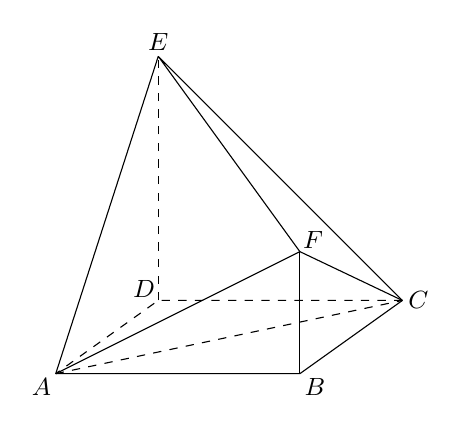
\begin{tikzpicture}[scale=1.55, font=\small]
  \coordinate (A) at (0,0);
  \coordinate (B) at (2,0);
  \coordinate (C) at (2.84,0.60);
  \coordinate (D) at (0.84,0.60);
  \coordinate (E) at (0.84,2.60);
  \coordinate (F) at (2,1.00);
  % 可见实线
  \draw (A) -- (B) -- (C);
  \draw (B) -- (F);
  \draw (E) -- (A)  (E) -- (C)  (E) -- (F);
  \draw (F) -- (A)  (F) -- (C);
  % 被遮挡
  \draw[dashed] (C) -- (D) -- (A);
  \draw[dashed] (A) -- (C);
  \draw[dashed] (D) -- (E);
  \node[below left,  inner sep=1.5pt] at (A) {$A$};
  \node[below right, inner sep=1.5pt] at (B) {$B$};
  \node[right,       inner sep=2pt]   at (C) {$C$};
  \node[above left,  inner sep=1pt]   at (D) {$D$};
  \node[above,       inner sep=2pt]   at (E) {$E$};
  \node[above right, inner sep=1pt]   at (F) {$F$};
\end{tikzpicture}
\end{center}
\nopagebreak[4]
\begin{gkopts}(4)
\task A．$V_3=2V_2$
\task B．$V_3=V_1$
\task C．$V_3=V_1+V_2$
\task D．$2V_3=3V_1$
\end{gkopts}

\Needspace{4\baselineskip}
\textbf{解析}

\textbf{第一步，建系（比例题，尺寸可自定）。}

四个选项都是体积之间的\textbf{倍数关系}，与绝对尺寸无关，故取
\nopagebreak[4]
\[AB=ED=2,\qquad FB=1\]

因 $ED\perp$ 平面 $ABCD$ 且 $FB\parallel ED$，故 $FB$ 也垂直于平面 $ABCD$。以 $A$ 为原点，$AB$、$AD$ 为 $x$、$y$ 轴，竖直方向为 $z$ 轴：
\nopagebreak[4]
\[A(0,0,0),\ B(2,0,0),\ C(2,2,0),\ D(0,2,0),\ E(0,2,2),\ F(2,0,1)\]

\textbf{第二步，逐个求体积。}

\textbf{$V_1=V_{E\text{-}ACD}$}：底面 $\triangle ACD$ 在平面 $z=0$ 内，面积 $=\dfrac12\times2\times2=2$；$E$ 到该平面的距离为 $ED=2$。
\nopagebreak[4]
\[V_1=\frac13\times2\times2=\frac43\]

\textbf{$V_2=V_{F\text{-}ABC}$}：底面 $\triangle ABC$ 面积 $=2$；$F$ 到平面 $ABCD$ 的距离为 $FB=1$。
\nopagebreak[4]
\[V_2=\frac13\times2\times1=\frac23\]

\textbf{$V_3=V_{F\text{-}ACE}$}：用行列式（混合积）公式
\nopagebreak[4]
\[V_3=\frac16\left|\det\left(\overrightarrow{AC},\ \overrightarrow{AE},\ \overrightarrow{AF}\right)\right|\]

\nopagebreak[4]
\[\overrightarrow{AC}=(2,2,0),\quad\overrightarrow{AE}=(0,2,2),\quad\overrightarrow{AF}=(2,0,1)\]

\nopagebreak[4]
\[\det=\begin{vmatrix}2&2&0\\0&2&2\\2&0&1\end{vmatrix}=2(2\times1-2\times0)-2(0\times1-2\times2)+0=4+8=12\]

\nopagebreak[4]
\[V_3=\frac{12}6=2\]

\textbf{汇总}：
\nopagebreak[4]
\[V_1=\frac43,\qquad V_2=\frac23,\qquad V_3=2\]

\textbf{第三步，逐项判断。}

\begin{itemize}
\item \textbf{A}：$2V_2=\dfrac43\ne2=V_3$  \textbf{错误}
\item \textbf{B}：$V_1=\dfrac43\ne2=V_3$  \textbf{错误}
\item \textbf{C}：$V_1+V_2=\dfrac43+\dfrac23=2=V_3$  \textbf{正确}
\item \textbf{D}：$2V_3=4$，$3V_1=3\times\dfrac43=4$，相等  \textbf{正确}
\end{itemize}

\begin{gktip}
\textbf{C 项的几何含义}：三个三棱锥 $F\text{-}ABC$、$E\text{-}ACD$、$F\text{-}ACE$ 恰好把整个多面体 $ABCDEF$（即六个点的凸包）\textbf{无重叠地剖分}——底面正方形被对角线 $AC$ 分成 $\triangle ABC$ 与 $\triangle ACD$ 两半，两半各自向上"顶起"一个三棱锥，剩下的空隙正是 $F\text{-}ACE$。故
\nopagebreak[4]
\[V_1+V_2+V_3=V_{ABCDEF}\]
程序用凸包蒙特卡洛测得 $V_{ABCDEF}=4.00$，而 $V_1+V_2+V_3=\dfrac43+\dfrac23+2=4$  剖分成立。但要由此\textbf{独立地}得出 $V_3=V_1+V_2$，仍需另行算出总体积 $V_{ABCDEF}=4$，并不比直接算 $V_3$ 省事。

\textbf{考场结论}：本题四个选项都要判断，\textbf{建系一次、把三个体积全部算出来}是最稳的路线；混合积（行列式）公式 $V=\dfrac16\left|\det\right|$ 让 $V_3$ 这种"没有现成底面高"的三棱锥也能一步得出。

\textbf{D 项的一句话看法}：$V_3=2=\dfrac32\times\dfrac43=\dfrac32V_1$，即 $2V_3=3V_1$。C、D 两项其实是同一组数据的两种写法，\textbf{同时成立并不矛盾}——多选题里"看起来互斥"的选项经常都对。
\end{gktip}

\gkanswer{答案：CD}

\par\medskip

\end{answer}
\begin{answer}
\gksolhead{12}{}

\textbf{题目}：

若 $x$，$y$ 满足 $x^{2}+y^{2}-xy=1$，则\mbox{（　　）}

\begin{gkopts}(2)
\task A．$x+y\le1$
\task B．$x+y\ge-2$
\task C．$x^{2}+y^{2}\le2$
\task D．$x^{2}+y^{2}\ge1$
\end{gkopts}

\Needspace{4\baselineskip}
\textbf{解析}

\textbf{核心技巧：换用和 $s=x+y$、积 $q=xy$ 这一对对称变量。}

\nopagebreak[4]
\[x^{2}+y^{2}=(x+y)^{2}-2xy=s^{2}-2q\]

代入条件：
\nopagebreak[4]
\[s^{2}-2q-q=1\ \Longrightarrow\ s^{2}-3q=1\ \Longrightarrow\ q=\frac{s^{2}-1}3\]

\textbf{关键约束}：$x$、$y$ 是实数 $\Leftrightarrow$ 它们是方程 $t^{2}-st+q=0$ 的两个实根 $\Leftrightarrow$ 判别式非负：
\nopagebreak[4]
\[s^{2}-4q\ge0\ \Longrightarrow\ s^{2}-\frac{4\left(s^{2}-1\right)}3\ge0\ \Longrightarrow\ 3s^{2}-4s^{2}+4\ge0\ \Longrightarrow\ s^{2}\le4\]

\nopagebreak[4]
\[\boxed{-2\le x+y\le2}\]

再把 $x^{2}+y^{2}$ 也用 $s$ 表示：
\nopagebreak[4]
\[x^{2}+y^{2}=1+q=1+\frac{s^{2}-1}3=\frac{s^{2}+2}3\]

由 $s^{2}\in[0,4]$：
\nopagebreak[4]
\[\boxed{\frac23\le x^{2}+y^{2}\le2}\]

两个区间的端点都能取到：

\begin{itemize}
\item $s=2$：$q=1$，$x=y=1$，此时 $x+y=2$、$x^{2}+y^{2}=2$；
\item $s=-2$：$x=y=-1$，$x+y=-2$、$x^{2}+y^{2}=2$；
\item $s=0$：$q=-\dfrac13$，$x=\dfrac1{\sqrt3}$、$y=-\dfrac1{\sqrt3}$，此时 $x^{2}+y^{2}=\dfrac23$。
\end{itemize}

\textbf{逐项判断}：

\begin{itemize}
\item \textbf{A}：$x+y\le1$？取 $x=y=1$ 得 $x+y=2>1$  \textbf{错误}
\item \textbf{B}：$x+y\ge-2$？由 $s\ge-2$  \textbf{正确}
\item \textbf{C}：$x^{2}+y^{2}\le2$？由上界  \textbf{正确}
\item \textbf{D}：$x^{2}+y^{2}\ge1$？取 $x=\dfrac1{\sqrt3}$、$y=-\dfrac1{\sqrt3}$ 得 $\dfrac23<1$  \textbf{错误}
\end{itemize}

\textbf{数值验证}：把约束曲线参数化为 $r^{2}(1-\sin\theta\cos\theta)=1$，扫描 $2\times10^{5}$ 个 $\theta$，得 $x+y\in[-2,2]$、$x^{2}+y^{2}\in[0.6667,2]$  与理论完全吻合。

\begin{gktip}
\textbf{方法总结}：$x^{2}+y^{2}-xy=1$ 是一个\textbf{椭圆}（长轴沿 $y=x$，短轴沿 $y=-x$）。三种主流解法：
1. \textbf{对称变量法}（上文）：一次换元同时解决两组选项，最推荐；
2. \textbf{参数法}：椭圆化标准形后设 $x=\sqrt2\cos t+\ldots$，计算量大；
3. \textbf{基本不等式法}：由 $xy\le\dfrac{(x+y)^{2}}4$ 得
\nopagebreak[4]
\[1=(x+y)^{2}-3xy\ge(x+y)^{2}-\frac34(x+y)^{2}=\frac14(x+y)^{2}\]
   同样给出 $(x+y)^{2}\le4$；至于 $x^{2}+y^{2}$ 的范围，则要分别用 $xy\le\dfrac{x^{2}+y^{2}}2$（得上界 $x^{2}+y^{2}\le2$）与 $xy\ge-\dfrac{x^{2}+y^{2}}2$（得下界 $x^{2}+y^{2}\ge\dfrac23$）\textbf{两次}，方向相反、\textbf{容易只做一边就下结论}。

\textbf{本题最大的陷阱是 D}：$x^{2}+y^{2}\ge1$ 在直觉上很"像"对的（毕竟等式右边是 $1$），但 $-xy$ 这一项在 $x$、$y$ 异号时是\textbf{正贡献}，会把 $x^{2}+y^{2}$ 压到 $1$ 以下。\textbf{看到 $\pm xy$ 交叉项，一定要分别检验同号与异号两种情形}。
\end{gktip}

\gkanswer{答案：BC}

\par\medskip

\end{answer}
\gkpart{三、填空题（每小题 5 分，共 20 分）}

\begin{answer}
\gksolhead{13}{}

\textbf{题目}：

已知随机变量 $X$ 服从正态分布 $N\left(2,\sigma^{2}\right)$，且 $P(2<X\le2.5)=0.36$，则 $P(X>2.5)=$ \gkblank{}．

\Needspace{4\baselineskip}
\textbf{解析}

\textbf{关键：正态曲线关于均值 $\mu=2$ 对称。}

对称性给出
\nopagebreak[4]
\[P(X>2)=P(X<2)=\frac12=0.5\]

把事件 $\{X>2\}$ 沿 $x=2.5$ 切成互斥的两块：
\nopagebreak[4]
\[\{X>2\}=\{2<X\le2.5\}\cup\{X>2.5\}\]

\nopagebreak[4]
\[P(X>2)=P(2<X\le2.5)+P(X>2.5)\]

\nopagebreak[4]
\[0.5=0.36+P(X>2.5)\]

\nopagebreak[4]
\[P(X>2.5)=0.5-0.36=0.14\]

\begin{gktip}
\textbf{提醒}：本题\textbf{根本用不到 $\sigma$}——题目给出 $\sigma^{2}$ 只是为了写全分布的名字。凡是"已知均值一侧某段概率、求同侧剩余部分"的正态题，都只需对称性 $+$ 加减，\textbf{看到 $\sigma$ 未知不要慌}。

\textbf{另一类常考变形}：若问 $P(X\le1.5)$，则用对称 $P(X\le1.5)=P(X\ge2.5)=0.14$（$1.5$ 与 $2.5$ 关于 $2$ 对称）。
\end{gktip}

\gkanswer{答案：$0.14$}

\par\medskip

\end{answer}
\begin{answer}
\gksolhead{14}{}

\textbf{题目}：

曲线 $y=\ln|x|$ 经过坐标原点的两条切线的方程分别为 \gkblank{}，\gkblank{}．

\Needspace{4\baselineskip}
\textbf{解析}

\textbf{注意定义域}：$y=\ln|x|$ 的定义域是 $x\ne0$，曲线由\textbf{两支}组成（$x>0$ 与 $x<0$），原点不在曲线上，所以是"过原点作切线"，切点未知，必须设。

\textbf{第一支（$x>0$）}：此时 $y=\ln x$，$y'=\dfrac1x$。

设切点为 $\left(t,\ \ln t\right)$（$t>0$），切线斜率 $\dfrac1t$。切线过原点意味着\textbf{切点与原点连线的斜率等于切线斜率}：
\nopagebreak[4]
\[\frac{\ln t-0}{t-0}=\frac1t\]

两边乘 $t$（$t>0$）：
\nopagebreak[4]
\[\ln t=1\ \Longrightarrow\ t=\mathrm e\]

切点 $(\mathrm e,1)$，斜率 $\dfrac1{\mathrm e}$：
\nopagebreak[4]
\[y=\frac1{\mathrm e}x\]

\textbf{第二支（$x<0$）}：此时 $y=\ln(-x)$，求导
\nopagebreak[4]
\[y'=\frac1{-x}\times(-1)=\frac1x\]

（导数形式与右支相同，这是 $\ln|x|$ 的一个便利性质。）

设切点 $\left(t,\ \ln(-t)\right)$（$t<0$）：
\nopagebreak[4]
\[\frac{\ln(-t)}{t}=\frac1t\ \Longrightarrow\ \ln(-t)=1\ \Longrightarrow\ -t=\mathrm e\ \Longrightarrow\ t=-\mathrm e\]

切点 $(-\mathrm e,1)$，斜率 $\dfrac1t=-\dfrac1{\mathrm e}$：
\nopagebreak[4]
\[y=-\frac1{\mathrm e}x\]

\textbf{验证}：$(\mathrm e,1)$ 满足 $y=\dfrac x{\mathrm e}$ ；$(-\mathrm e,1)$ 满足 $y=-\dfrac x{\mathrm e}$ ；两条切线都过原点 

\begin{gktip}
\textbf{对称性速解}：$y=\ln|x|$ 是\textbf{偶函数}，图象关于 $y$ 轴对称。所以只要求出右支的切线 $y=\dfrac x{\mathrm e}$，左支的切线就是它关于 $y$ 轴的镜像 $y=-\dfrac x{\mathrm e}$，\textbf{第二支根本不用再算一遍}。

\textbf{易错点}：把题目看成 $y=\ln x$ 而只答一条。题干明写"两条切线"，绝对值符号是本题的全部信息量所在。
\end{gktip}

\gkanswer{答案：$y=\dfrac1{\mathrm e}x$ 与 $y=-\dfrac1{\mathrm e}x$}

\par\medskip

\end{answer}
\begin{answer}
\gksolhead{15}{}

\textbf{题目}：

设点 $A(-2,3)$，$B(0,a)$，若直线 $AB$ 关于 $y=a$ 对称的直线与圆 $(x+3)^{2}+(y+2)^{2}=1$ 有公共点，则 $a$ 的取值范围是 \gkblank{}．

\Needspace{4\baselineskip}
\textbf{解析}

\textbf{第一步，求出对称后的直线。}

对称轴是水平线 $y=a$。

\begin{itemize}
\item $B(0,a)$ \textbf{在对称轴上}，对称后不动，仍是 $B(0,a)$；
\item $A(-2,3)$ 的对称点：横坐标不变，纵坐标满足"到 $y=a$ 距离相等且异侧"，即 $y_{A'}=2a-3$，故
\end{itemize}
\nopagebreak[4]
\[A'(-2,\ 2a-3)\]

对称后的直线就是过 $A'$ 与 $B$ 的直线。

\textbf{第二步，写出该直线的方程。}

斜率：
\nopagebreak[4]
\[k=\frac{a-(2a-3)}{0-(-2)}=\frac{3-a}2\]

（分母恒为 $2\ne0$，所以这条直线\textbf{永远不是竖直线}，无需讨论。）

由点斜式（过 $B(0,a)$）：
\nopagebreak[4]
\[y=\frac{3-a}2x+a\]

整理成一般式（两边乘 $2$ 后移项）：
\nopagebreak[4]
\[(3-a)x-2y+2a=0\]

\textbf{第三步，"有公共点"化为圆心到直线的距离条件。}

圆心 $(-3,-2)$，半径 $r=1$。直线与圆有公共点（相交或相切）等价于
\nopagebreak[4]
\[d=\frac{|(3-a)(-3)-2\times(-2)+2a|}{\sqrt{(3-a)^{2}+(-2)^{2}}}\le1\]

\textbf{先化简分子}：
\nopagebreak[4]
\[(3-a)(-3)+4+2a=-9+3a+4+2a=5a-5=5(a-1)\]

\nopagebreak[4]
\[d=\frac{5|a-1|}{\sqrt{(a-3)^{2}+4}}\le1\]

\textbf{第四步，去分母求解。}

两边非负，可平方：
\nopagebreak[4]
\[25(a-1)^{2}\le(a-3)^{2}+4\]

\nopagebreak[4]
\[25a^{2}-50a+25\le a^{2}-6a+9+4\]

\nopagebreak[4]
\[24a^{2}-44a+12\le0\]

同除 $4$：
\nopagebreak[4]
\[6a^{2}-11a+3\le0\]

因式分解（$6\times3=18$，凑 $-9$ 与 $-2$）：
\nopagebreak[4]
\[(3a-1)(2a-3)\le0\]

\nopagebreak[4]
\[\frac13\le a\le\frac32\]

\textbf{数值验证}：在 $[-3,4]$ 上以步长 $10^{-5}$ 扫描 $a$，满足 $d\le1$ 的 $a$ 恰好落在 $[0.33334,\ 1.5]$ 内 （下端 $0.33334$ 即 $\dfrac13$ 的离散化）

\begin{gktip}
\textbf{本题的三个易错处}：
1. \textbf{只反射一个点就够了}——$B$ 在对称轴上是不动点，很多人把两个点都反射，结果 $B$ 被错误地搬到 $(0,a)$ 的"对称位置"$(0,a)$……虽然结果相同，但若把 $B$ 误认为要变，容易顺手写错。\textbf{先判断哪些点在轴上}。
2. \textbf{"有公共点"是 $d\le r$，不是 $d<r$}——相切也算有公共点，端点 $\dfrac13$ 与 $\dfrac32$ 必须闭。
3. \textbf{分子的绝对值不能提前去掉}——$5(a-1)$ 在 $a<1$ 时为负，平方后才安全。
\end{gktip}

\gkanswer{答案：$\left[\dfrac13,\dfrac32\right]$}

\par\medskip

\end{answer}
\begin{answer}
\gksolhead{16}{}

\textbf{题目}：

已知直线 $l$ 与椭圆 $\dfrac{x^{2}}6+\dfrac{y^{2}}3=1$ 在第一象限交于 $A$，$B$ 两点，$l$ 与 $x$ 轴、$y$ 轴分别交于 $M$，$N$ 两点，且 $|MA|=|NB|$，$|MN|=2\sqrt3$，则 $l$ 的方程为 \gkblank{}．

\Needspace{4\baselineskip}
\textbf{解析}

\textbf{第一步，把 $|MA|=|NB|$ 翻译成"中点重合"。}

$M$、$N$、$A$、$B$ 四点都在直线 $l$ 上。因 $A$、$B$ 在第一象限而 $M$ 在 $x$ 轴、$N$ 在 $y$ 轴，$l$ 的斜率必为负，四点沿 $l$ 的排列顺序是 $N,\ B,\ A,\ M$。

两端的线段等长 $|NB|=|AM|$，故\textbf{线段 $AB$ 与线段 $MN$ 有相同的中点}（把 $N$、$M$ 各向内移动同样的距离得到 $B$、$A$）。

\textbf{第二步，设直线并写两个中点。}

设 $l:y=kx+m$（$k<0$，$m>0$）。

\begin{itemize}
\item $M$（令 $y=0$）：$\left(-\dfrac mk,\ 0\right)$；$N$（令 $x=0$）：$(0,\ m)$。
\end{itemize}
\nopagebreak[4]
\[\text{\text{中点}}_{MN}=\left(-\frac m{2k},\ \frac m2\right)\]

\begin{itemize}
\item 联立椭圆：把 $y=kx+m$ 代入 $\dfrac{x^{2}}6+\dfrac{y^{2}}3=1$，两边乘 $6$：
\end{itemize}
\nopagebreak[4]
\[x^{2}+2(kx+m)^{2}=6\ \Longrightarrow\ \left(1+2k^{2}\right)x^{2}+4kmx+2m^{2}-6=0\]

  由韦达定理 $x_A+x_B=-\dfrac{4km}{1+2k^{2}}$：
\nopagebreak[4]
\[\text{\text{中点}}_{AB}\text{ \text{的横坐标}}=-\frac{2km}{1+2k^{2}}\]

\textbf{第三步，令两个中点的横坐标相等。}
\nopagebreak[4]
\[-\frac{2km}{1+2k^{2}}=-\frac m{2k}\]

$m\ne0$（否则直线过原点，$M=N=O$，$|MN|=0$），约去 $m$ 并交叉相乘：
\nopagebreak[4]
\[4k^{2}=1+2k^{2}\ \Longrightarrow\ k^{2}=\frac12\]

由 $k<0$：
\nopagebreak[4]
\[k=-\frac{\sqrt2}2\]

\textbf{第四步，用 $|MN|=2\sqrt3$ 定 $m$。}
\nopagebreak[4]
\[|MN|^{2}=\left(\frac mk\right)^{2}+m^{2}=m^{2}\left(\frac1{k^{2}}+1\right)=m^{2}(2+1)=3m^{2}\]

\nopagebreak[4]
\[3m^{2}=\left(2\sqrt3\right)^{2}=12\ \Longrightarrow\ m^{2}=4\ \Longrightarrow\ m=\pm2\]

$m=-2$ 时直线 $y=-\dfrac{\sqrt2}2x-2$ 与第一象限无交点（$x>0$ 时 $y<-2<0$），舍去。故 $m=2$：
\nopagebreak[4]
\[l:\ y=-\frac{\sqrt2}2x+2\]

\textbf{第五步，回代验证（必做）。}

代入判别式方程：$\left(1+2\times\dfrac12\right)x^{2}+4\times\left(-\dfrac{\sqrt2}2\right)\times2\cdot x+2\times4-6=0$，即
\nopagebreak[4]
\[2x^{2}-4\sqrt2x+2=0\ \Longrightarrow\ x^{2}-2\sqrt2x+1=0\]

\nopagebreak[4]
\[x=\frac{2\sqrt2\pm\sqrt{8-4}}2=\sqrt2\pm1\]

两根都为正；对应
\nopagebreak[4]
\[y=-\frac{\sqrt2}2\left(\sqrt2+1\right)+2=1-\frac{\sqrt2}2\approx0.293>0\]
\nopagebreak[4]
\[y=-\frac{\sqrt2}2\left(\sqrt2-1\right)+2=1+\frac{\sqrt2}2\approx1.707>0\]

\textbf{两交点确实都在第一象限} 

再核对：$M=\left(2\sqrt2,0\right)$、$N=(0,2)$，$|MN|=\sqrt{8+4}=2\sqrt3$ ；程序算得 $|MA|=|NB|=0.507307$ 

\begin{gktip}
\textbf{核心一步是"$|MA|=|NB|\Leftrightarrow$ 中点重合"}。这个转化把一个含根号的长度等式变成了一个只用韦达定理的坐标等式，是圆锥曲线中"\textbf{等长弦}"类问题的通法：
\nopagebreak[4]
\[|MA|=|NB|\iff\overrightarrow{MA}=\overrightarrow{NB}\iff A-M=B-N\iff\frac{A+B}2=\frac{M+N}2\]
\textbf{注意}：这一步用到了两条线段\textbf{同向}（由四点顺序保证），若 $A$、$B$ 不都在第一象限，顺序可能变化，等价性就要重新论证。

\textbf{另一个观察}：本题的 $k^{2}=\dfrac12$ 恰好等于 $\dfrac{b^{2}}{a^{2}}=\dfrac36=\dfrac12$。这不是巧合——"椭圆的弦中点与坐标轴截距中点重合"这一条件化简后必然给出 $k^{2}=\dfrac{b^{2}}{a^{2}}$，\textbf{换个椭圆做同类题时可以直接套}。
\end{gktip}

\gkanswer{答案：$y=-\dfrac{\sqrt2}2x+2$}

\par\medskip

\end{answer}
\gkpart{四、解答题（共 70 分）}

\begin{answer}
\gksolhead{17}{10 分}

\textbf{题目}（10 分）：

已知 $\left\{a_n\right\}$ 是等差数列，$\left\{b_n\right\}$ 是公比为 $2$ 的等比数列，且 $a_2-b_2=a_3-b_3=b_4-a_4$。

  (1) 证明：$a_1=b_1$；

  (2) 求集合 $\left\{k\mid b_k=a_m+a_1,\ 1\le m\le500\right\}$ 中元素的个数。

\Needspace{4\baselineskip}
\textbf{解析}

\par\medskip

\textbf{(1) 证明}

\textbf{设参数}：设 $\left\{a_n\right\}$ 的首项为 $a_1$、公差为 $d$，$\left\{b_n\right\}$ 的首项为 $b_1$、公比为 $2$。于是
\nopagebreak[4]
\[a_n=a_1+(n-1)d,\qquad b_n=b_1\cdot2^{\,n-1}\]

\textbf{写出题给的三个量}：
\nopagebreak[4]
\[a_2-b_2=\left(a_1+d\right)-2b_1\]
\nopagebreak[4]
\[a_3-b_3=\left(a_1+2d\right)-4b_1\]
\nopagebreak[4]
\[b_4-a_4=8b_1-\left(a_1+3d\right)\]

\textbf{由前两式相等}：
\nopagebreak[4]
\[a_1+d-2b_1=a_1+2d-4b_1\]

消去 $a_1$，移项：
\nopagebreak[4]
\[2b_1=d\qquad(\text{i})\]

\textbf{由后两式相等}：
\nopagebreak[4]
\[a_1+2d-4b_1=8b_1-a_1-3d\]

\nopagebreak[4]
\[2a_1+5d=12b_1\qquad(\text{ii})\]

\textbf{把 (i) 代入 (ii)}（$d=2b_1$）：
\nopagebreak[4]
\[2a_1+10b_1=12b_1\ \Longrightarrow\ 2a_1=2b_1\ \Longrightarrow\ a_1=b_1\qquad\blacksquare\]

\textbf{验证}：取 $b_1=a_1=1$，则 $d=2$，$a_n=2n-1$，$b_n=2^{\,n-1}$。
\nopagebreak[4]
\[a_2-b_2=3-2=1,\quad a_3-b_3=5-4=1,\quad b_4-a_4=8-7=1\]
三者确实相等 

\par\medskip

\textbf{(2) 解}

\textbf{第一步，把 $a_m+a_1$ 和 $b_k$ 都写成 $b_1$ 的倍数。}

由 (1) 记 $a_1=b_1=:t$（等比数列要求 $t\ne0$），由 $(\text i)$ 有 $d=2t$，故
\nopagebreak[4]
\[a_m=t+(m-1)\cdot2t=(2m-1)t\]

\nopagebreak[4]
\[a_m+a_1=(2m-1)t+t=2mt\]

\nopagebreak[4]
\[b_k=t\cdot2^{\,k-1}\]

\textbf{第二步，解方程 $b_k=a_m+a_1$。}
\nopagebreak[4]
\[t\cdot2^{\,k-1}=2mt\]

约去 $t\ne0$：
\nopagebreak[4]
\[2^{\,k-1}=2m\ \Longrightarrow\ m=2^{\,k-2}\]

\textbf{第三步，找出满足约束的 $k$。}

需要 $m$ 是\textbf{正整数}且 $1\le m\le500$：

\begin{itemize}
\item $k=1$：$m=2^{-1}=\dfrac12$，\textbf{不是整数}，舍；
\item $k=2$：$m=2^{0}=1$ 
\item $k=3$：$m=2$ 
\item $\cdots$
\item $k=10$：$m=2^{8}=256\le500$ 
\item $k=11$：$m=2^{9}=512>500$ ，此后更大，全部不合。
\end{itemize}

故
\nopagebreak[4]
\[k\in\{2,3,4,5,6,7,8,9,10\}\]

\textbf{第四步，计数。}
\nopagebreak[4]
\[10-2+1=9\]

\textbf{程序验证}：取 $t=1$，对 $k=1,\dots,59$ 逐一搜索是否存在 $1\le m\le500$ 使 $b_k=a_m+a_1$，得到的 $k$ 恰为 $\{2,3,\dots,10\}$，共 $9$ 个 

\textbf{该集合中元素的个数为 $9$。}

\begin{gktip}
\textbf{方法总结}：
1. \textbf{(1) 问的本质是"两个方程解两个未知量"}——三个量两两相等给出 2 个方程，未知量是 $d$ 与 $b_1$（相对于 $a_1$ 的比例），恰好定解。不要试图把 $a_1$ 也解出来：题目条件对 $a_1$ 是齐次的，$a_1$ 可以任意（只要 $\ne0$）。
2. \textbf{(2) 问的关键是把常数 $t$ 约掉}——所有量都正比于 $t$，方程 $2^{k-1}=2m$ 与 $t$ 无关，说明\textbf{答案与数列的具体首项无关}，这也解释了为什么题目不给具体数值。
3. \textbf{计数时的两个边界都要单独验}：下界 $k=1$ 因 $m$ 不是整数而失效（\textbf{不是因为 $m$ 越界}），上界 $k=11$ 因 $m>500$ 而失效。$2^{8}=256$、$2^{9}=512$ 这两个数卡在 $500$ 两侧，是命题人刻意设计的。
\end{gktip}

\gkanswer{答案（1）：见解析版}

\gkanswer{答案（2）：$9$ 个}

\par\medskip

\end{answer}
\begin{answer}
\gksolhead{18}{12 分}

\textbf{题目}（12 分）：

记 $\triangle ABC$ 的内角 $A$，$B$，$C$ 的对边分别为 $a$，$b$，$c$，分别以 $a$，$b$，$c$ 为边长的三个正三角形的面积依次为 $S_1$，$S_2$，$S_3$。已知 $S_1-S_2+S_3=\dfrac{\sqrt3}2$，$\sin B=\dfrac13$。

  (1) 求 $\triangle ABC$ 的面积；

  (2) 若 $\sin A\sin C=\dfrac{\sqrt2}3$，求 $b$。

\Needspace{4\baselineskip}
\textbf{解析}

\par\medskip

\textbf{预备：把条件翻译成边的关系}

边长为 $s$ 的正三角形，面积为 $\dfrac{\sqrt3}4s^{2}$。故
\nopagebreak[4]
\[S_1=\frac{\sqrt3}4a^{2},\qquad S_2=\frac{\sqrt3}4b^{2},\qquad S_3=\frac{\sqrt3}4c^{2}\]

条件 $S_1-S_2+S_3=\dfrac{\sqrt3}2$ 变成
\nopagebreak[4]
\[\frac{\sqrt3}4\left(a^{2}-b^{2}+c^{2}\right)=\frac{\sqrt3}2\]

两边同除 $\dfrac{\sqrt3}4$：
\nopagebreak[4]
\[a^{2}+c^{2}-b^{2}=2\qquad(\ast)\]

\textbf{这个组合正是余弦定理的左边}：
\nopagebreak[4]
\[a^{2}+c^{2}-b^{2}=2ac\cos B\]

于是
\nopagebreak[4]
\[2ac\cos B=2\ \Longrightarrow\ ac\cos B=1\qquad(\ast\ast)\]

\par\medskip

\textbf{(1) 解}

\textbf{第一步，定 $\cos B$ 的符号。}

由 $(\ast\ast)$，$ac>0$ 故 $\cos B>0$，即 $B$ 为\textbf{锐角}（这一步不能省——$\sin B=\dfrac13$ 本身允许 $B$ 为钝角）。

\nopagebreak[4]
\[\cos B=\sqrt{1-\sin^{2}B}=\sqrt{1-\frac19}=\frac{2\sqrt2}3\]

\textbf{第二步，求 $ac$。}

代入 $(\ast\ast)$：
\nopagebreak[4]
\[ac\times\frac{2\sqrt2}3=1\ \Longrightarrow\ ac=\frac3{2\sqrt2}=\frac{3\sqrt2}4\]

\textbf{第三步，求面积。}
\nopagebreak[4]
\[S_{\triangle ABC}=\frac12ac\sin B=\frac12\times\frac{3\sqrt2}4\times\frac13=\frac{\sqrt2}8\]

\par\medskip

\textbf{(2) 解}

\textbf{第一步，用正弦定理把 $\sin A\sin C$ 换成 $ac$。}

设外接圆半径为 $R$，则 $a=2R\sin A$、$c=2R\sin C$，故
\nopagebreak[4]
\[ac=4R^{2}\sin A\sin C\]

代入已知 $\sin A\sin C=\dfrac{\sqrt2}3$ 与 (1) 中的 $ac=\dfrac{3\sqrt2}4$：
\nopagebreak[4]
\[\frac{3\sqrt2}4=4R^{2}\times\frac{\sqrt2}3\]

\nopagebreak[4]
\[4R^{2}=\frac{3\sqrt2}4\times\frac3{\sqrt2}=\frac94\]

\textbf{第二步，求 $b$。}

由正弦定理 $b=2R\sin B$，即 $b^{2}=4R^{2}\sin^{2}B$：
\nopagebreak[4]
\[b^{2}=\frac94\times\frac19=\frac14\ \Longrightarrow\ b=\frac12\]

\textbf{完整验算（构造出这个三角形）}：

由 $\sin A\sin C=\dfrac12\left[\cos(A-C)-\cos(A+C)\right]$ 且 $A+C=\pi-B$：
\nopagebreak[4]
\[\frac{\sqrt2}3=\frac12\left[\cos(A-C)+\cos B\right]=\frac12\left[\cos(A-C)+\frac{2\sqrt2}3\right]\]

\nopagebreak[4]
\[\cos(A-C)=\frac{2\sqrt2}3-\frac{2\sqrt2}3=0\ \Longrightarrow\ |A-C|=\frac\pi2\]

于是 $B=\arcsin\dfrac13\approx19.4712^\circ$，$A\approx125.2644^\circ$，$C\approx35.2644^\circ$。取 $R=\dfrac34$ 算出
\nopagebreak[4]
\[a\approx1.224745,\quad b=0.5,\quad c\approx0.866025\]

回代检验：
\nopagebreak[4]
\[\frac{\sqrt3}4\left(a^{2}-b^{2}+c^{2}\right)\approx0.8660254=\frac{\sqrt3}2\ \]
\nopagebreak[4]
\[\sin A\sin C\approx0.4714045=\frac{\sqrt2}3\ ,\qquad S=\frac12ac\sin B\approx0.1767767=\frac{\sqrt2}8\ \]

\begin{gktip}
\textbf{方法总结}：
1. \textbf{"正三角形面积"只是余弦定理的伪装}。看到 $S_1-S_2+S_3$ 这种\textbf{带正负号的组合}，先把公共系数 $\dfrac{\sqrt3}4$ 提出来，剩下的 $a^{2}-b^{2}+c^{2}$ 立刻暴露出余弦定理的身影。命题人用几何外衣包装代数恒等式，是近年解三角形题的常见手法。
2. \textbf{$\cos B$ 的正负必须由条件确定，不能默认}。本题靠 $ac\cos B=1>0$ 排除钝角。若漏掉这一步而取 $\cos B=-\dfrac{2\sqrt2}3$，会得到 $ac<0$ 的荒谬结果。
3. \textbf{(2) 问的路线是"边 $\to$ 角 $\to$ 边"}：已知 $ac$（边的积）与 $\sin A\sin C$（角的积），二者通过 $4R^{2}$ 相连，求出 $4R^{2}$ 后再回到 $b=2R\sin B$。\textbf{整道题始终没有单独求出 $a$ 或 $c$}，这正是正弦定理"整体代换"的威力。
\end{gktip}

\gkanswer{答案（1）：$\dfrac{\sqrt2}8$}

\gkanswer{答案（2）：$b=\dfrac12$}

\par\medskip

\end{answer}
\begin{answer}
\gksolhead{19}{12 分}

\textbf{题目}（12 分）：

在某地区进行流行病学调查，随机调查了 $100$ 位某种疾病患者的年龄，得到如下的样本数据的频率分布直方图。
\nopagebreak[4]
\begin{center}% 2022 新高考Ⅱ卷 19：年龄频率分布直方图
% 九组，组距均为 10（[0,10),…,[80,90)），频率/组距依次为
% 0.001、0.002、0.012、0.017、0.023、0.020、0.017、0.006、0.002（合计 ×10 = 1）。
% 纵轴刻度自下而上 0.001、0.002、0.006、0.012、0.017、0.020、0.023，各引水平虚线至对应矩形顶。
\begin{tikzpicture}[font=\small, x=0.088cm, y=260cm]
  % ---- 引至矩形顶的水平虚线 ----
  \draw[dashed] (0,0.001) -- (10,0.001);
  \draw[dashed] (0,0.002) -- (20,0.002);
  \draw[dashed] (0,0.006) -- (80,0.006);
  \draw[dashed] (0,0.012) -- (30,0.012);
  \draw[dashed] (0,0.017) -- (40,0.017);
  \draw[dashed] (0,0.020) -- (60,0.020);
  \draw[dashed] (0,0.023) -- (50,0.023);
  % ---- 直方图矩形 ----
  \draw ( 0,0) rectangle (10,0.001);
  \draw (10,0) rectangle (20,0.002);
  \draw (20,0) rectangle (30,0.012);
  \draw (30,0) rectangle (40,0.017);
  \draw (40,0) rectangle (50,0.023);
  \draw (50,0) rectangle (60,0.020);
  \draw (60,0) rectangle (70,0.017);
  \draw (70,0) rectangle (80,0.006);
  \draw (80,0) rectangle (90,0.002);
  % ---- 坐标轴 ----
  \draw[-stealth] (0,0) -- (97,0);
  \draw[-stealth] (0,0) -- (0,0.0258);
  % ---- 刻度 ----
  \foreach \x in {10,20,30,40,50,60,70,80,90}
    { \draw (\x,0) -- (\x,-0.00035); \node[below, inner sep=2pt] at (\x,-0.0002) {\footnotesize $\x$}; }
  \foreach \y/\lab in {0.001/0.001,0.002/0.002,0.006/0.006,0.012/0.012,0.017/0.017,0.020/0.020,0.023/0.023}
    { \draw (0,\y) -- (-1.6,\y); \node[left, inner sep=2pt] at (-1.6,\y) {\footnotesize $\lab$}; }
  \node[below left, inner sep=1.5pt] at (0,0) {$0$};
  % ---- 轴名 ----
  \node[right, inner sep=3pt] at (97,0) {年龄/岁};
  \node[above, inner sep=2.5pt] at (0,0.0258) {$\displaystyle\frac{\mbox{频率}}{\mbox{组距}}$};
\end{tikzpicture}
\end{center}
\nopagebreak[4]
  (1) 估计该地区这种疾病患者的平均年龄；（同一组中的数据用该区间的中点值为代表）

  (2) 估计该地区一位这种疾病患者的年龄位于区间 $[20,70)$ 的概率；

  (3) 已知该地区这种疾病患者的患病率为 $0.1\%$，该地区年龄位于区间 $[40,50)$ 的人口占该地区总人口的 $16\%$。从该地区中任选一人，若此人的年龄位于区间 $[40,50)$，求此人患这种疾病的概率。（以样本数据中患者的年龄位于各区间的频率作为患者的年龄位于该区间的概率，精确到 $0.0001$）

\Needspace{4\baselineskip}
\textbf{解析}

(1) 估计该地区这种疾病患者的平均年龄；（同一组中的数据用该区间的中点值为代表）(2) 估计该地区一位这种疾病患者的年龄位于区间 $[20,70)$ 的概率；(3) 已知该地区这种疾病患者的患病率为 $0.1\%$，该地区年龄位于区间 $[40,50)$ 的人口占该地区总人口的 $16\%$。从该地区中任选一人，若此人的年龄位于区间 $[40,50)$，求此人患这种疾病的概率。（以样本数据中患者的年龄位于各区间的频率作为患者的年龄位于该区间的概率，精确到 $0.0001$）

\par\medskip

\textbf{预备：把直方图读成频率表}

直方图纵轴是 $\dfrac{\text{\text{频率}}}{\text{\text{组距}}}$，组距为 $10$，故\textbf{频率 = 纵轴读数 $\times10$}：

\begin{center}
\begingroup\setlength{\tabcolsep}{4pt}
\begin{tabular}{cccccccccc}
\toprule
年龄区间 & $[0,10)$ & $[10,20)$ & $[20,30)$ & $[30,40)$ & $[40,50)$ & $[50,60)$ & $[60,70)$ & $[70,80)$ & $[80,90)$ \\
\midrule
频率/组距 & $0.001$ & $0.002$ & $0.012$ & $0.017$ & $0.023$ & $0.020$ & $0.017$ & $0.006$ & $0.002$ \\
频率 & $0.01$ & $0.02$ & $0.12$ & $0.17$ & $0.23$ & $0.20$ & $0.17$ & $0.06$ & $0.02$ \\
组中值 & $5$ & $15$ & $25$ & $35$ & $45$ & $55$ & $65$ & $75$ & $85$ \\
\bottomrule
\end{tabular}
\endgroup
\end{center}

\textbf{自检}：所有频率之和
\nopagebreak[4]
\[0.01+0.02+0.12+0.17+0.23+0.20+0.17+0.06+0.02=1.00\ \]

（这一步务必先做——若和不为 $1$，说明读图有误，后面全错。）

\par\medskip

\textbf{(1) 解}

平均年龄 $=\sum(\text{\text{组中值}}\times\text{\text{频率}})$：
\nopagebreak[4]
\[\bar x=5\times0.01+15\times0.02+25\times0.12+35\times0.17+45\times0.23\]
\nopagebreak[4]
\[\qquad+55\times0.20+65\times0.17+75\times0.06+85\times0.02\]

逐项：
\nopagebreak[4]
\[0.05+0.30+3.00+5.95+10.35+11.00+11.05+4.50+1.70\]

累加：
\nopagebreak[4]
\[0.05+0.30=0.35;\ +3.00=3.35;\ +5.95=9.30;\ +10.35=19.65;\]
\nopagebreak[4]
\[+11.00=30.65;\ +11.05=41.70;\ +4.50=46.20;\ +1.70=47.90\]

\nopagebreak[4]
\[\bar x=47.9\]

\par\medskip

\textbf{(2) 解}

$[20,70)$ 覆盖 $[20,30)$、$[30,40)$、$[40,50)$、$[50,60)$、$[60,70)$ 五组，概率即这五组频率之和：
\nopagebreak[4]
\[P=0.12+0.17+0.23+0.20+0.17=0.89\]

（\textbf{验算捷径}：用补集更快——$1-(0.01+0.02+0.06+0.02)=1-0.11=0.89$ ）

\par\medskip

\textbf{(3) 解}

\textbf{第一步，设事件、翻译已知。}

设
\begin{itemize}
\item $C=$"此人患这种疾病"，
\item $D=$"此人年龄位于 $[40,50)$"。
\end{itemize}

题目给出：
\nopagebreak[4]
\[P(C)=0.1\%=0.001,\qquad P(D)=16\%=0.16\]

而"以样本数据中患者的年龄位于各区间的频率作为患者的年龄位于该区间的概率"这句话的含义是：\textbf{在患者中}，年龄落在 $[40,50)$ 的比例即为直方图对应的频率
\nopagebreak[4]
\[P(D\mid C)=0.23\]

\textbf{第二步，用条件概率公式（贝叶斯）。}
\nopagebreak[4]
\[P(C\mid D)=\frac{P(CD)}{P(D)}=\frac{P(D\mid C)P(C)}{P(D)}\]

\textbf{第三步，代入。}
\nopagebreak[4]
\[P(C\mid D)=\frac{0.23\times0.001}{0.16}=\frac{0.00023}{0.16}=0.0014375\]

按题目要求精确到 $0.0001$：
\nopagebreak[4]
\[P(C\mid D)\approx0.0014\]

\begin{gktip}
\textbf{方法总结}：
1. \textbf{直方图题的第一动作永远是"验证频率和为 $1$"}。本题九个矩形高度中有 $0.001$、$0.002$ 这类小值，读图时极易与 $0.01$、$0.02$ 混淆；和为 $1$ 这一校验能当场抓住读错。
2. \textbf{(3) 问的题眼是分清"谁是条件"}：直方图描述的是\textbf{患者}这个总体的年龄分布，所以它给的是 $P(\text{\text{年龄}}\mid\text{\text{患病}})$ 而不是 $P(\text{\text{患病}}\mid\text{\text{年龄}})$。题目要求的恰是反过来的那一个，必须用贝叶斯公式\textbf{掉个头}。混淆这两者是流行病学统计中最经典的错误（"基础率谬误"）。
3. \textbf{结果的量级值得回味}：$[40,50)$ 岁人群的患病率 $0.0014$ 是全人群患病率 $0.001$ 的 $1.4375$ 倍——恰好等于 $\dfrac{0.23}{0.16}$，即"患者中该年龄段占比"与"总人口中该年龄段占比"之比。这个比值就是流行病学中的\textbf{富集倍数}，可作为答案的快速自检。
\end{gktip}

\gkanswer{答案（1）：$47.9$ 岁}

\gkanswer{答案（2）：$0.89$}

\gkanswer{答案（3）：约 $0.0014$}

\par\medskip

\end{answer}
\begin{answer}
\gksolhead{20}{12 分}

\textbf{题目}（12 分）：

如图，$PO$ 是三棱锥 $P\text{-}ABC$ 的高，$PA=PB$，$AB\perp AC$，$E$ 为 $PB$ 的中点。
\nopagebreak[4]
\begin{center}% 2022 新高考Ⅱ卷 20：三棱锥 P-ABC（PO⊥底面 ABC，E 为 PB 的中点）
% 立体坐标 A(0,0,0)、B(4√3,0,0)、C(0,12,0)、O(2√3,2,0)、P(2√3,2,3)、E(3√3,1,3/2)。
% 画布投影：(x,y,z) -> x·(1,0) + y·(-0.22,0.46) + z·(0,1)，故 C 落在左上远处、O 在底面内部、P 在 O 正上方。
% 深度方向取得较陡，是为了让汇于远点 C 的五条连线张开成可辨的扇形。
% 虚线（被遮挡）：PO（竖直）、CB、CO、CE；其余为可见实线。
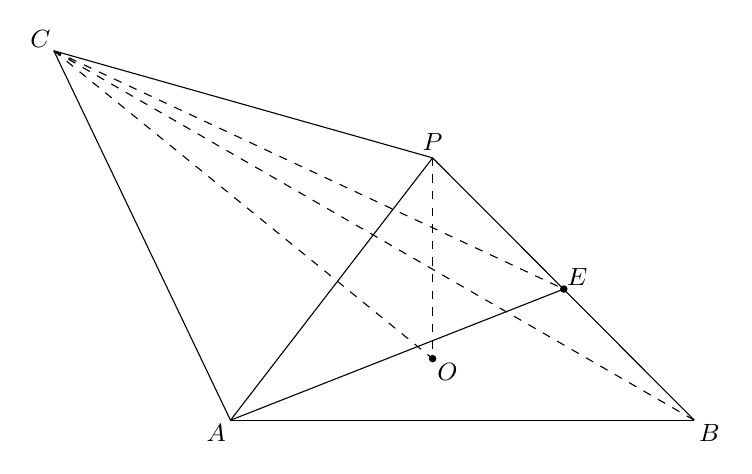
\begin{tikzpicture}[scale=0.85, font=\small]
  \coordinate (A) at (0,0);
  \coordinate (B) at (6.93,0);
  \coordinate (C) at (-2.64,5.52);
  \coordinate (O) at (3.02,0.92);
  \coordinate (P) at (3.02,3.92);
  \coordinate (E) at (4.98,1.96);
  % 可见实线
  \draw (A) -- (B);
  \draw (A) -- (C);
  \draw (P) -- (A)  (P) -- (B)  (P) -- (C);
  \draw (A) -- (E);
  % 被遮挡
  \draw[dashed] (P) -- (O);
  \draw[dashed] (C) -- (B)  (C) -- (O)  (C) -- (E);
  \fill (O) circle (1.6pt);
  \fill (E) circle (1.6pt);
  \node[below left,  inner sep=1.5pt] at (A) {$A$};
  \node[below right, inner sep=1.5pt] at (B) {$B$};
  \node[above left,  inner sep=1pt]   at (C) {$C$};
  \node[below right, inner sep=1.5pt] at (O) {$O$};
  \node[above,       inner sep=2.5pt] at (P) {$P$};
  \node[above right, inner sep=1pt]   at (E) {$E$};
\end{tikzpicture}
\end{center}
\nopagebreak[4]
  (1) 证明：$OE\parallel$ 平面 $PAC$；

  (2) 若 $\angle ABO=\angle CBO=30^\circ$，$PO=3$，$PA=5$，求二面角 $C\text{-}AE\text{-}B$ 正弦值。

\Needspace{4\baselineskip}
\textbf{解析}

(1) 证明：$OE\parallel$ 平面 $PAC$；(2) 若 $\angle ABO=\angle CBO=30^\circ$，$PO=3$，$PA=5$，求二面角 $C\text{-}AE\text{-}B$ 正弦值。

\par\medskip

\textbf{(1) 证明}

\textbf{第一步，由 $PA=PB$ 推出 $OA=OB$。}

"$PO$ 是三棱锥的高"即 $PO\perp$ 平面 $ABC$，故 $PO\perp OA$、$PO\perp OB$。

在两个直角三角形中用勾股定理：
\nopagebreak[4]
\[OA^{2}=PA^{2}-PO^{2},\qquad OB^{2}=PB^{2}-PO^{2}\]

由 $PA=PB$ 立得
\nopagebreak[4]
\[OA=OB\]

\textbf{第二步，取 $AB$ 中点 $D$，搭出一个平行于平面 $PAC$ 的平面。}

设 $D$ 为 $AB$ 的中点，连 $OD$、$DE$。

\begin{itemize}
\item \textbf{$OD\parallel AC$}：由 $OA=OB$ 知 $\triangle OAB$ 是等腰三角形，中线 $OD\perp AB$；又已知 $AC\perp AB$，同一平面（平面 $ABC$）内垂直于同一条直线的两条直线平行，故 $OD\parallel AC$。
\end{itemize}

\begin{itemize}
\item \textbf{$DE\parallel PA$}：在 $\triangle ABP$ 中，$D$、$E$ 分别是 $AB$、$PB$ 的中点，$DE$ 是中位线。
\end{itemize}

\textbf{第三步，由线线平行升级为面面平行。}

$AC\subset$ 平面 $PAC$ 且 $OD\not\subset$ 平面 $PAC$，故 $OD\parallel$ 平面 $PAC$；

$PA\subset$ 平面 $PAC$ 且 $DE\not\subset$ 平面 $PAC$，故 $DE\parallel$ 平面 $PAC$。

（\textbf{关于"不在平面内"的确认}：若 $O$ 在平面 $PAC$ 内，则 $O$ 在平面 $PAC$ 与平面 $ABC$ 的交线 $AC$ 上；由 $OD\parallel AC$ 且 $O\in AC$ 得直线 $OD$ 与 $AC$ 重合，于是中点 $D\in AC$。但 $D\in AB$ 且 $AB\cap AC=\{A\}$，只能 $D=A$，即 $B=A$，与三棱锥矛盾。故 $O\notin$ 平面 $PAC$，同理 $D$、$E$ 也不在其中。）

$OD$ 与 $DE$ 是平面 $ODE$ 内两条相交直线（交于 $D$），且都平行于平面 $PAC$，故
\nopagebreak[4]
\[\text{\text{平面} }ODE\parallel\text{\text{平面} }PAC\]

\textbf{第四步，收尾。}

$OE\subset$ 平面 $ODE$，而平面 $ODE\parallel$ 平面 $PAC$，故
\nopagebreak[4]
\[OE\parallel\text{\text{平面} }PAC\qquad\blacksquare\]

\par\medskip

\textbf{(2) 解}

\textbf{第一步，把所有长度算出来。}

在 $\mathrm{Rt}\triangle POA$ 中（$PO\perp OA$）：
\nopagebreak[4]
\[OA=\sqrt{PA^{2}-PO^{2}}=\sqrt{25-9}=4\]

由 (1) 的结论 $OB=OA=4$。

$\triangle OAB$ 等腰，两底角相等，而 $\angle ABO=30^\circ$，故 $\angle OAB=30^\circ$、$\angle AOB=120^\circ$。底边
\nopagebreak[4]
\[AB=2\times OB\times\cos30^\circ=2\times4\times\frac{\sqrt3}2=4\sqrt3\]

由 $\angle ABO=\angle CBO=30^\circ$（$BO$ 是 $\angle ABC$ 的平分线）：
\nopagebreak[4]
\[\angle ABC=30^\circ+30^\circ=60^\circ\]

在 $\mathrm{Rt}\triangle BAC$ 中（直角在 $A$）：
\nopagebreak[4]
\[AC=AB\tan\angle ABC=4\sqrt3\times\sqrt3=12\]

\textbf{第二步，建立空间直角坐标系。}

以 $A$ 为原点，$\overrightarrow{AB}$ 为 $x$ 轴正方向，$\overrightarrow{AC}$ 为 $y$ 轴正方向（$AB\perp AC$ 保证二者垂直），竖直向上为 $z$ 轴：
\nopagebreak[4]
\[A(0,0,0),\qquad B\left(4\sqrt3,0,0\right),\qquad C(0,12,0)\]

\textbf{定 $O$ 的坐标}：$O$ 在平面 $ABC$（即 $z=0$）内，且 $OA=OB=4$。由 $OA=OB$ 知 $O$ 的横坐标是 $A$、$B$ 横坐标的平均值 $2\sqrt3$；再由 $OA=4$：
\nopagebreak[4]
\[\left(2\sqrt3\right)^{2}+y_O^{2}=16\ \Longrightarrow\ y_O^{2}=4\ \Longrightarrow\ y_O=\pm2\]

$BO$ 平分 $\angle ABC$，$O$ 应与 $C$ 在 $AB$ 的同侧，取 $y_O=2$：
\nopagebreak[4]
\[O\left(2\sqrt3,\ 2,\ 0\right),\qquad P=O+(0,0,PO)=\left(2\sqrt3,\ 2,\ 3\right)\]

\textbf{校验}：$PA=\sqrt{12+4+9}=\sqrt{25}=5$ ；$PB=\sqrt{\left(2\sqrt3-4\sqrt3\right)^{2}+4+9}=\sqrt{12+13}=5$ ；$\angle ABO$、$\angle CBO$ 用向量算得均为 $30.0000^\circ$ 

\textbf{第三步，定 $E$ 并求两个半平面的法向量。}

$E$ 为 $PB$ 的中点：
\nopagebreak[4]
\[E=\frac{P+B}2=\left(\frac{2\sqrt3+4\sqrt3}2,\ \frac{2+0}2,\ \frac{3+0}2\right)=\left(3\sqrt3,\ 1,\ \frac32\right)\]

二面角 $C\text{-}AE\text{-}B$ 的棱是 $AE$，两个半平面分别含 $C$ 和 $B$，即平面 $AEC$ 与平面 $AEB$。

\nopagebreak[4]
\[\overrightarrow{AE}=\left(3\sqrt3,1,\frac32\right),\qquad\overrightarrow{AC}=(0,12,0),\qquad\overrightarrow{AB}=\left(4\sqrt3,0,0\right)\]

\textbf{平面 $AEC$ 的法向量}：
\nopagebreak[4]
\[\boldsymbol n_1=\overrightarrow{AE}\times\overrightarrow{AC}=\left(1\times0-\frac32\times12,\frac32\times0-3\sqrt3\times0,3\sqrt3\times12-1\times0\right)=\left(-18,0,36\sqrt3\right)\]

\textbf{平面 $AEB$ 的法向量}：
\nopagebreak[4]
\[\boldsymbol n_2=\overrightarrow{AE}\times\overrightarrow{AB}=\left(1\times0-\frac32\times0,\frac32\times4\sqrt3-3\sqrt3\times0,0-1\times4\sqrt3\right)=\left(0,6\sqrt3,-4\sqrt3\right)\]

\textbf{第四步，求夹角。}
\nopagebreak[4]
\[\boldsymbol n_1\cdot\boldsymbol n_2=(-18)\times0+0\times6\sqrt3+36\sqrt3\times\left(-4\sqrt3\right)=-432\]

\nopagebreak[4]
\[\left|\boldsymbol n_1\right|=\sqrt{324+0+3888}=\sqrt{4212}=\sqrt{4\times1053}=2\sqrt{1053}=2\times9\sqrt{13}=18\sqrt{13}\]

\nopagebreak[4]
\[\left|\boldsymbol n_2\right|=\sqrt{0+108+48}=\sqrt{156}=2\sqrt{39}\]

\nopagebreak[4]
\[\cos\theta=\frac{-432}{18\sqrt{13}\times2\sqrt{39}}=\frac{-432}{36\sqrt{507}}=\frac{-12}{\sqrt{507}}\]

因 $507=169\times3$，$\sqrt{507}=13\sqrt3$：
\nopagebreak[4]
\[\cos\theta=\frac{-12}{13\sqrt3}=-\frac{12\sqrt3}{39}=-\frac{4\sqrt3}{13}\]

\textbf{第五步，求正弦值。}
\nopagebreak[4]
\[\sin\theta=\sqrt{1-\cos^{2}\theta}=\sqrt{1-\frac{48}{169}}=\sqrt{\frac{121}{169}}=\frac{11}{13}\]

\textbf{（正弦值与二面角是钝角还是锐角无关，$\cos$ 的符号不影响结论。）}

\textbf{程序核验}：$\cos\theta=-0.53293871=-\dfrac{4\sqrt3}{13}$ ，$\sin\theta=0.84615385=\dfrac{11}{13}$ ；同时验证 $\overrightarrow{OE}\cdot\boldsymbol n_{PAC}=0$（即 (1) 的结论）

\begin{gktip}
\textbf{方法总结}：
1. \textbf{(1) 问的钥匙是"三棱锥的高"这五个字}——它等价于 $PO\perp$ 平面 $ABC$，从而两个直角三角形共用直角边 $PO$，由 $PA=PB$ 得 $OA=OB$。这是全题唯一的隐藏条件，读题时必须立刻兑现。
2. \textbf{证线面平行时"造中位线"是首选}，但本题的巧妙在于 $OE$ 自身找不到平行线，必须\textbf{借第三点 $D$（$AB$ 中点）搭出一个平行平面}。"线面平行难证时，升级为面面平行"是立体几何的常规迂回。
3. \textbf{(2) 问建系的难点是定位 $O$}：$O$ 不在任何一条棱上，需要用 $OA=OB$（横坐标居中）与 $OA=4$（到 $A$ 的距离）两个条件联立，并用 $BO$ 平分 $\angle ABC$ 定符号。\textbf{$y_O=\pm2$ 的取舍不能凭感觉，要说明理由。}
4. \textbf{$\sqrt{4212}$ 这类大根号一定要分解质因数化简}（$4212=4\times1053=4\times81\times13$），否则最后一步的约分无从下手。
\end{gktip}

\gkanswer{答案（1）：见解析版}

\gkanswer{答案（2）：$\dfrac{11}{13}$}

\par\medskip

\end{answer}
\begin{answer}
\gksolhead{21}{12 分}

\textbf{题目}（12 分）：

已知双曲线 $C:\dfrac{x^{2}}{a^{2}}-\dfrac{y^{2}}{b^{2}}=1\ (a>0,\ b>0)$ 的右焦点为 $F(2,0)$，渐近线方程为 $y=\pm\sqrt3x$。

  (1) 求 $C$ 的方程；

  (2) 过 $F$ 的直线与 $C$ 的两条渐近线分别交于 $A$，$B$ 两点，点 $P\left(x_1,y_1\right)$，$Q\left(x_2,y_2\right)$ 在 $C$ 上，且 $x_1>x_2>0$，$y_1>0$。过 $P$ 且斜率为 $-\sqrt3$ 的直线与过 $Q$ 且斜率为 $\sqrt3$ 的直线交于点 $M$。从下面①②③中选取两个作为条件，证明另外一个成立。

  　① $M$ 在 $AB$ 上；② $PQ\parallel AB$；③ $|MA|=|MB|$。

\Needspace{4\baselineskip}
\textbf{解析}

\par\medskip

\textbf{(1) 解}

渐近线斜率 $\dfrac ba=\sqrt3$，即 $b=\sqrt3a$，故 $b^{2}=3a^{2}$。

右焦点 $F(2,0)$ 给出 $c=2$，而 $c^{2}=a^{2}+b^{2}$：
\nopagebreak[4]
\[4=a^{2}+3a^{2}=4a^{2}\ \Longrightarrow\ a^{2}=1,\qquad b^{2}=3\]

\nopagebreak[4]
\[C:\ x^{2}-\frac{y^{2}}3=1\]

\par\medskip

\textbf{(2) 关键工具：改用"渐近线坐标"}

\textbf{动机}：本题中出现的一切直线，斜率不是 $\sqrt3$ 就是 $-\sqrt3$——\textbf{正好是两条渐近线的斜率}。把渐近线当作新的"坐标轴"，所有条件都会变得极其简洁。

\textbf{定义}（对平面上任一点 $(x,y)$）：
\nopagebreak[4]
\[u=\sqrt3x-y,\qquad v=\sqrt3x+y\]

这是一个可逆线性变换，逆变换为
\nopagebreak[4]
\[x=\frac{u+v}{2\sqrt3},\qquad y=\frac{v-u}2\]

线性变换把直线映成直线、把中点映成中点、把平行映成平行，故与"共线""平行""中点"有关的条件可以直接在 $(u,v)$ 中判断。

\textbf{四条基本事实}：

1. \textbf{点在 $C$ 上 $\iff uv=3$}：
\nopagebreak[4]
\[uv=\left(\sqrt3x-y\right)\left(\sqrt3x+y\right)=3x^{2}-y^{2}=3\left(x^{2}-\frac{y^{2}}3\right)=3\]

2. \textbf{斜率 $-\sqrt3$ 的直线 $\iff v=$ 常数}（沿该直线 $\mathrm dv=\sqrt3\,\mathrm dx+\mathrm dy=\sqrt3\,\mathrm dx-\sqrt3\,\mathrm dx=0$）；
   \textbf{斜率 $\sqrt3$ 的直线 $\iff u=$ 常数}。

3. \textbf{渐近线}：$y=\sqrt3x\iff u=0$；$y=-\sqrt3x\iff v=0$。

4. \textbf{长度}：对向量 $(\Delta u,\Delta v)$，其在原坐标下的长度平方为
\nopagebreak[4]
\[\Delta x^{2}+\Delta y^{2}=\frac{(\Delta u+\Delta v)^{2}}{12}+\frac{(\Delta v-\Delta u)^{2}}4=\frac{\Delta u^{2}-\Delta u\Delta v+\Delta v^{2}}3\]

\textbf{设点}：记
\nopagebreak[4]
\[P:\left(u_1,v_1\right),\quad Q:\left(u_2,v_2\right),\qquad u_1v_1=u_2v_2=3\]

不妨设 $A$ 在渐近线 $u=0$ 上、$B$ 在渐近线 $v=0$ 上：
\nopagebreak[4]
\[A:(0,\ \alpha),\qquad B:(\beta,\ 0)\]

\textbf{$M$ 的坐标}：过 $P$ 且斜率 $-\sqrt3$ 的直线是 $v=v_1$；过 $Q$ 且斜率 $\sqrt3$ 的直线是 $u=u_2$。两者交于
\nopagebreak[4]
\[\boxed{M:\left(u_2,\ v_1\right)}\]

（两直线斜率不同，交点必存在且唯一。）

\textbf{符号约定}：由 $x_1>x_2>0$ 知 $P$、$Q$ 都在右支上。右支上 $uv=3>0$ 且 $u+v=2\sqrt3x>0$，故
\nopagebreak[4]
\[u_1,\ v_1,\ u_2,\ v_2>0\]

又 $u_2v_1\ne3$：否则 $u_2=\dfrac3{v_1}=u_1$ 且 $v_2=\dfrac3{u_2}=v_1$，即 $Q=P$，与 $x_1>x_2$ 矛盾。

\par\medskip

\textbf{三个条件的代数刻画}

\textbf{② $PQ\parallel AB$}

$PQ$ 的方向向量（用 $u_1=\dfrac3{v_1}$、$v_2=\dfrac3{u_2}$）：
\nopagebreak[4]
\[\left(u_2-u_1,\ v_2-v_1\right)=\left(\frac{u_2v_1-3}{v_1},\ \frac{3-u_2v_1}{u_2}\right)=\left(u_2v_1-3\right)\left(\frac1{v_1},\ -\frac1{u_2}\right)\]

由于 $u_2v_1-3\ne0$ 且 $u_2v_1>0$，方向向量与 $\left(u_2,\ -v_1\right)$ 平行（把括号内的向量乘以 $u_2v_1$）：
\nopagebreak[4]
\[\overrightarrow{PQ}\parallel\left(u_2,\ -v_1\right)\]

$AB$ 的方向向量：$\overrightarrow{AB}=(\beta,-\alpha)$。故
\nopagebreak[4]
\[\text{②}\iff u_2(-\alpha)-\left(-v_1\right)\beta=0\iff\frac\beta{u_2}=\frac\alpha{v_1}\]

记这个公共比值为 $\lambda$，即 \textbf{② $\iff\beta=\lambda u_2$ 且 $\alpha=\lambda v_1$}。

\textbf{① $M$ 在 $AB$ 上}

直线 $AB$ 的截距式为 $\dfrac u\beta+\dfrac v\alpha=1$（$\alpha,\beta\ne0$，否则 $A$、$B$ 重合于原点，与"交于两点"矛盾）。代入 $M\left(u_2,v_1\right)$：
\nopagebreak[4]
\[\text{①}\iff\frac{u_2}\beta+\frac{v_1}\alpha=1\]

\textbf{③ $|MA|=|MB|$}

\nopagebreak[4]
\[\overrightarrow{MA}=\left(-u_2,\ \alpha-v_1\right),\qquad\overrightarrow{MB}=\left(\beta-u_2,\ -v_1\right)\]

由长度公式（事实 4）：
\nopagebreak[4]
\[3|MA|^{2}=u_2^{2}+u_2\left(\alpha-v_1\right)+\left(\alpha-v_1\right)^{2}\]
\nopagebreak[4]
\[3|MB|^{2}=\left(\beta-u_2\right)^{2}+\left(\beta-u_2\right)v_1+v_1^{2}\]

\par\medskip

\textbf{证明三个方向}

\textbf{（甲）由①②证③}

由②：$\beta=\lambda u_2$、$\alpha=\lambda v_1$。代入①：
\nopagebreak[4]
\[\frac{u_2}{\lambda u_2}+\frac{v_1}{\lambda v_1}=\frac1\lambda+\frac1\lambda=\frac2\lambda=1\ \Longrightarrow\ \lambda=2\]

于是 $\beta=2u_2$、$\alpha=2v_1$，即
\nopagebreak[4]
\[M\left(u_2,v_1\right)=\left(\frac{0+\beta}2,\ \frac{\alpha+0}2\right)=\text{\text{线段} }AB\text{ \text{的中点}}\]

（中点在线性变换下保持，故在原坐标下 $M$ 也是 $AB$ 的中点。）中点到两端点距离相等：
\nopagebreak[4]
\[|MA|=|MB|\qquad\blacksquare\]

\textbf{（乙）由①③证②}

①说明 $A$、$M$、$B$ 三点共线，③说明 $M$ 到 $A$、$B$ 距离相等。共线且等距 $\Rightarrow$ $M$ 是\textbf{线段 $AB$ 的中点}（$A\ne B$）。于是
\nopagebreak[4]
\[u_2=\frac{0+\beta}2\ \Longrightarrow\ \beta=2u_2,\qquad v_1=\frac{\alpha+0}2\ \Longrightarrow\ \alpha=2v_1\]

\nopagebreak[4]
\[\overrightarrow{AB}=(\beta,-\alpha)=\left(2u_2,\ -2v_1\right)=2\left(u_2,-v_1\right)\parallel\overrightarrow{PQ}\]

故 $PQ\parallel AB$（且 $PQ$ 与 $AB$ 不重合：$P$、$Q$ 在双曲线上，$A$、$B$ 在渐近线上，若两线重合则渐近线与双曲线相交，矛盾）$\qquad\blacksquare$

\textbf{（丙）由②③证①}

由②记 $\beta=\lambda u_2$、$\alpha=\lambda v_1$，代入两个长度式：
\nopagebreak[4]
\[3|MA|^{2}=u_2^{2}+(\lambda-1)u_2v_1+(\lambda-1)^{2}v_1^{2}\]
\nopagebreak[4]
\[3|MB|^{2}=(\lambda-1)^{2}u_2^{2}+(\lambda-1)u_2v_1+v_1^{2}\]

作差（中间项相同，相消）：
\nopagebreak[4]
\[3\left(|MA|^{2}-|MB|^{2}\right)=\left(u_2^{2}-v_1^{2}\right)-\left(\lambda-1\right)^{2}\left(u_2^{2}-v_1^{2}\right)=\left(u_2^{2}-v_1^{2}\right)\left[1-(\lambda-1)^{2}\right]\]

由③得
\nopagebreak[4]
\[\left(u_2^{2}-v_1^{2}\right)\left[1-(\lambda-1)^{2}\right]=0\]

\textbf{排除第一个因子为零}：$u_2,v_1>0$ 故 $u_2\ne-v_1$；若 $u_2=v_1$，则
\nopagebreak[4]
\[u_1=\frac3{v_1}=\frac3{u_2}=v_2\]
\nopagebreak[4]
\[x_1=\frac{u_1+v_1}{2\sqrt3}=\frac{v_2+u_2}{2\sqrt3}=x_2\]
与 $x_1>x_2$ 矛盾。故 $u_2^{2}\ne v_1^{2}$。

因此
\nopagebreak[4]
\[(\lambda-1)^{2}=1\ \Longrightarrow\ \lambda=2\ \text{\text{或}}\ \lambda=0\]

$\lambda=0$ 给出 $\alpha=\beta=0$，即 $A=B=$ 原点，与"交于 $A$、$B$ 两点"矛盾，舍。故 $\lambda=2$，从而
\nopagebreak[4]
\[\frac{u_2}\beta+\frac{v_1}\alpha=\frac12+\frac12=1\]

即 $M$ 在直线 $AB$ 上 $\qquad\blacksquare$

\par\medskip

\textbf{数值验证（取①②为条件的一组具体数据）}

再加上"$AB$ 过 $F(2,0)$"这一条件（$F$ 在新坐标下是 $\left(2\sqrt3,2\sqrt3\right)$），代入 $\dfrac{2\sqrt3}\beta+\dfrac{2\sqrt3}\alpha=1$ 与 $\beta=2u_2$、$\alpha=2v_1$ 得
\nopagebreak[4]
\[\frac{\sqrt3}{u_2}+\frac{\sqrt3}{v_1}=1\]

取 $u_2=3$，解得 $v_1=\dfrac{\sqrt3}{1-\frac{\sqrt3}3}\approx4.098076$。由此
\nopagebreak[4]
\[P\approx(1.394338,\ 1.683013),\quad Q\approx(1.154701,\ -1),\quad M\approx(2.049038,\ 0.549038)\]
\nopagebreak[4]
\[A\approx(2.366025,\ 4.098076),\quad B\approx(1.732051,\ -3)\]

程序核验：$P$、$Q$ 都满足 $x^{2}-\dfrac{y^{2}}3=1$ ；$x_1>x_2>0$、$y_1>0$ ；$AB$ 过 $F$ ；$PM$ 斜率 $=-1.732051=-\sqrt3$、$QM$ 斜率 $=1.732051=\sqrt3$ ；$M$ 在 $AB$ 上 ；$PQ\parallel AB$ ；$|MA|=|MB|=3.56316607$ 。另在 $200$ 组随机参数上重复该检验，\textbf{无一例外} 

\begin{gktip}
\textbf{方法总结}：
1. \textbf{本题的破题点是"斜率 $\pm\sqrt3$ 恰为渐近线斜率"}。一旦意识到这一点，就应当想到用 $u=\sqrt3x-y$、$v=\sqrt3x+y$ 这组"渐近线坐标"（也叫\textbf{斜坐标}）改写全部条件：双曲线变成反比例曲线 $uv=3$，两族直线变成 $u=$ 常数与 $v=$ 常数，$M$ 的坐标一眼可见。若用常规的联立消元，本题的代数量将极其庞大。
2. \textbf{三个条件的等价核心是同一个数 $\lambda$}（$AB$ 相对于 $M$ 的"伸缩比"）：②把 $A$、$B$ 与 $M$ 绑定成比例 $\lambda$，①与③各自都等价于 $\lambda=2$，即"\textbf{$M$ 是 $AB$ 的中点}"。因此三条命题实际上共享一个几何本质——\textbf{$M$ 恰为弦 $AB$ 的中点}。看穿这一点，三个方向的证明就都只是同一件事的不同排列。
3. \textbf{不要忽略退化情形的排除}：$\lambda=0$（$A$、$B$ 重合于原点）与 $u_2=v_1$（$P$、$Q$ 横坐标相同）这两个分支都必须用题设的 $x_1>x_2>0$ 显式排除，否则（丙）的推理不成立。\textbf{"从①②③中选两个"型的证明题，评分点往往就在这些排除上。}
4. \textbf{有趣的旁证}：上面三个方向的推理\textbf{都没有用到"$AB$ 过 $F$"}。也就是说，该结论对任何与两条渐近线相交的直线 $AB$ 都成立；焦点条件只是把 $A$、$B$ 限定在一族具体的直线上，保证题目有确定的图形。
\end{gktip}

\gkanswer{答案（1）：$x^{2}-\dfrac{y^{2}}3=1$}

\gkanswer{答案（2）：见解析版}

\par\medskip

\end{answer}
\begin{answer}
\gksolhead{22}{12 分}

\textbf{题目}（12 分）：

已知函数 $f(x)=x\mathrm e^{ax}-\mathrm e^{x}$。

  (1) 当 $a=1$ 时，讨论 $f(x)$ 的单调性；

  (2) 当 $x>0$ 时，$f(x)<-1$，求 $a$ 的取值范围；

  (3) 设 $n\in\mathbf N^{*}$，证明：$\dfrac1{\sqrt{1^{2}+1}}+\dfrac1{\sqrt{2^{2}+2}}+\cdots+\dfrac1{\sqrt{n^{2}+n}}>\ln(n+1)$。

\par\medskip

\begin{gktip}
\textbf{试题来源}：deekur/gaokaomath（commit \texttt{34c13a6}，CC BY 4.0）之 \texttt{2022新高考2} PDF。
\end{gktip}

\Needspace{4\baselineskip}
\textbf{解析}

\par\medskip

\textbf{(1) 解}

$a=1$ 时
\nopagebreak[4]
\[f(x)=x\mathrm e^{x}-\mathrm e^{x}=(x-1)\mathrm e^{x}\]

求导（乘积法则）：
\nopagebreak[4]
\[f'(x)=1\cdot\mathrm e^{x}+(x-1)\mathrm e^{x}=x\mathrm e^{x}\]

因 $\mathrm e^{x}>0$ 恒成立，$f'(x)$ 的符号完全由 $x$ 决定：

\begin{itemize}
\item $x<0$ 时 $f'(x)<0$，$f(x)$ \textbf{单调递减}；
\item $x>0$ 时 $f'(x)>0$，$f(x)$ \textbf{单调递增}。
\end{itemize}

\textbf{结论：$f(x)$ 在 $(-\infty,0)$ 上单调递减，在 $(0,+\infty)$ 上单调递增（$x=0$ 处取极小值 $f(0)=-1$）。}

\textbf{数值核验}：$f'(-2)=-0.270671<0$、$f'(-0.5)=-0.303265<0$、$f'(0.5)=0.824361>0$、$f'(2)=14.778112>0$ 

\begin{gktip}
注意 $f(0)=-1$ 这个极小值——它正是 (2) 问要求 $f(x)<-1$ 的临界线索。
\end{gktip}

\par\medskip

\textbf{(2) 解}

\textbf{改写目标}：令
\nopagebreak[4]
\[g(x)=x\mathrm e^{ax}-\mathrm e^{x}+1\]

要求：\textbf{对一切 $x>0$ 有 $g(x)<0$}。

注意
\nopagebreak[4]
\[g(0)=0-1+1=0\]

即 $x=0$ 是"边界点"，问题变成"$g$ 从 $0$ 出发后能否始终待在 $0$ 以下"。

\par\medskip

\textbf{第一步（必要性）：证明必须有 $a\le\dfrac12$。}

对 $g$ 求两次导：
\nopagebreak[4]
\[g'(x)=\mathrm e^{ax}+ax\mathrm e^{ax}-\mathrm e^{x}=(1+ax)\mathrm e^{ax}-\mathrm e^{x}\]
\nopagebreak[4]
\[g''(x)=a\mathrm e^{ax}+a(1+ax)\mathrm e^{ax}-\mathrm e^{x}=\left(2a+a^{2}x\right)\mathrm e^{ax}-\mathrm e^{x}\]

在 $x=0$ 处：
\nopagebreak[4]
\[g(0)=0,\qquad g'(0)=1-1=0,\qquad g''(0)=2a-1\]

\textbf{反证}：假设 $a>\dfrac12$，则 $g''(0)=2a-1>0$。由 $g''$ 连续，存在 $\delta>0$ 使 $x\in[0,\delta)$ 时 $g''(x)>0$。于是：

\begin{itemize}
\item $g'$ 在 $[0,\delta)$ 上递增，结合 $g'(0)=0$ 得 $x\in(0,\delta)$ 时 $g'(x)>0$；
\item 进而 $g$ 在 $[0,\delta)$ 上递增，结合 $g(0)=0$ 得 $x\in(0,\delta)$ 时 $g(x)>0$。
\end{itemize}

这与"$x>0$ 时 $g(x)<0$"矛盾。故必有
\nopagebreak[4]
\[a\le\frac12\]

\par\medskip

\textbf{第二步（充分性）：证明 $a\le\dfrac12$ 时结论成立。}

\textbf{先把 $a$ 放大到 $\dfrac12$}：当 $x>0$ 且 $a\le\dfrac12$ 时，$ax\le\dfrac x2$，由指数函数单调递增
\nopagebreak[4]
\[x\mathrm e^{ax}\le x\mathrm e^{x/2}\]

因此只需证明\textbf{最强的情形}：
\nopagebreak[4]
\[x\mathrm e^{x/2}<\mathrm e^{x}-1\qquad(x>0)\]

\textbf{换元}：令 $t=\mathrm e^{x/2}$，则 $x>0\iff t>1$，且 $x=2\ln t$、$\mathrm e^{x}=t^{2}$。不等式变为
\nopagebreak[4]
\[2t\ln t<t^{2}-1\]

两边除以 $2t>0$：
\nopagebreak[4]
\[\ln t<\frac{t^{2}-1}{2t}=\frac12\left(t-\frac1t\right)\]

\textbf{证明这个不等式}：令
\nopagebreak[4]
\[h(t)=\frac12\left(t-\frac1t\right)-\ln t\qquad(t\ge1)\]

\nopagebreak[4]
\[h(1)=\frac12(1-1)-0=0\]

\nopagebreak[4]
\[h'(t)=\frac12\left(1+\frac1{t^{2}}\right)-\frac1t=\frac{t^{2}+1-2t}{2t^{2}}=\frac{(t-1)^{2}}{2t^{2}}\]

$t>1$ 时 $h'(t)>0$，故 $h$ 在 $[1,+\infty)$ 上严格递增，于是 $t>1$ 时
\nopagebreak[4]
\[h(t)>h(1)=0\ \Longrightarrow\ \ln t<\frac12\left(t-\frac1t\right)\]

代回即得 $x\mathrm e^{x/2}<\mathrm e^{x}-1$，从而对一切 $a\le\dfrac12$、$x>0$：
\nopagebreak[4]
\[x\mathrm e^{ax}\le x\mathrm e^{x/2}<\mathrm e^{x}-1\ \Longrightarrow\ f(x)=x\mathrm e^{ax}-\mathrm e^{x}<-1\]

\textbf{数值核验}（在 $x\in(0,8]$ 上取 $2\times10^{5}$ 个点求 $g$ 的最大值）：

\begin{center}
\begingroup\setlength{\tabcolsep}{4pt}
\begin{tabular}{cccccccc}
\toprule
$a$ & $-2$ & $0$ & $0.49$ & $0.5$ & $0.51$ & $0.6$ & $1$ \\
\midrule
$\max g$ & $-2.5\times10^{-12}$ & $-5.0\times10^{-13}$ & $-1.0\times10^{-14}$ & $0$（极限） & $9.3\times10^{-5}$ & $0.255$ & $2.1\times10^{4}$ \\
\bottomrule
\end{tabular}
\endgroup
\end{center}

分界线恰在 $a=\dfrac12$：$a\le0.5$ 时 $g$ 全程非正（$a=0.5$ 时上确界 $0$ 在 $x\to0^{+}$ 处取不到，故 $x>0$ 时仍严格小于 $0$），$a=0.51$ 起出现正值 

\par\medskip

\textbf{(3) 证明}

\textbf{思路}：把 (2) 在 $a=\dfrac12$ 时得到的不等式当作\textbf{工具}，对每个 $k$ 用一次，再求和。

\textbf{第一步，写出工具不等式。}

由 (2)（取 $a=\dfrac12$）：
\nopagebreak[4]
\[x\mathrm e^{x/2}<\mathrm e^{x}-1\qquad(x>0)\]

\textbf{第二步，选取合适的 $x$。}

对每个 $k\in\mathbf N^{*}$，取
\nopagebreak[4]
\[x=\ln\frac{k+1}k>0\]

（因 $\dfrac{k+1}k>1$，对数为正，符合 $x>0$ 的要求。）

此时
\nopagebreak[4]
\[\mathrm e^{x}=\frac{k+1}k,\qquad\mathrm e^{x/2}=\sqrt{\frac{k+1}k}\]

代入工具不等式：
\nopagebreak[4]
\[\ln\frac{k+1}k\cdot\sqrt{\frac{k+1}k}<\frac{k+1}k-1=\frac1k\]

\textbf{第三步，整理成目标形式。}

两边除以 $\sqrt{\dfrac{k+1}k}>0$：
\nopagebreak[4]
\[\ln\frac{k+1}k<\frac1k\cdot\sqrt{\frac k{k+1}}=\frac{\sqrt k}{k\sqrt{k+1}}=\frac1{\sqrt k\cdot\sqrt{k+1}}=\frac1{\sqrt{k(k+1)}}=\frac1{\sqrt{k^{2}+k}}\]

即对一切正整数 $k$：
\nopagebreak[4]
\[\ln\frac{k+1}k<\frac1{\sqrt{k^{2}+k}}\qquad(\dagger)\]

\textbf{第四步，对 $k=1,2,\dots,n$ 求和。}

左边\textbf{裂项相消}（对数把商变成差）：
\nopagebreak[4]
\[\sum_{k=1}^{n}\ln\frac{k+1}k=\sum_{k=1}^{n}\left[\ln(k+1)-\ln k\right]=\ln(n+1)-\ln1=\ln(n+1)\]

右边即待证的和。由 $(\dagger)$ 逐项严格小于：
\nopagebreak[4]
\[\ln(n+1)<\sum_{k=1}^{n}\frac1{\sqrt{k^{2}+k}}=\frac1{\sqrt{1^{2}+1}}+\frac1{\sqrt{2^{2}+2}}+\cdots+\frac1{\sqrt{n^{2}+n}}\qquad\blacksquare\]

\textbf{数值核验}：

\begin{center}
\begingroup\setlength{\tabcolsep}{4pt}
\begin{tabular}{cccccccc}
\toprule
$n$ & $1$ & $2$ & $3$ & $5$ & $10$ & $50$ & $200$ \\
\midrule
左边（和） & $0.70710$ & $1.11535$ & $1.40403$ & $1.81021$ & $2.41675$ & $3.95084$ & $5.32233$ \\
$\ln(n+1)$ & $0.69314$ & $1.09861$ & $1.38629$ & $1.79175$ & $2.39789$ & $3.93182$ & $5.30330$ \\
\bottomrule
\end{tabular}
\endgroup
\end{center}

每一行都是"和 $>$ 对数" ；另在 $k=1,\dots,1999$ 上逐个核验 $(\dagger)$ 全部成立 

\begin{gktip}
\textbf{方法总结}：
1. \textbf{(2) 问的标准结构是"必要性探路 + 充分性回证"}。必要性用\textbf{端点的二阶导}（$g(0)=g'(0)=0$，于是 $g''(0)$ 的符号决定 $g$ 在 $0$ 右侧的走向）快速锁定分界值 $a=\dfrac12$；充分性则把 $a$ 放大到分界值，化为一个单变量不等式。\textbf{没有必要性那一步，就只能靠猜测分界值。}
2. \textbf{换元 $t=\mathrm e^{x/2}$ 是充分性证明的关键}——它把混杂着 $x$、$\mathrm e^{x/2}$、$\mathrm e^{x}$ 的不等式统一成关于 $t$ 的初等不等式 $\ln t<\dfrac12\left(t-\dfrac1t\right)$，而后者的导数恰好是完全平方 $\dfrac{(t-1)^{2}}{2t^{2}}$，一眼可判正负。这条不等式本身值得背下来（它比常用的 $\ln t<t-1$ \textbf{更强}）。
3. \textbf{(3) 问是"用前问的结论造不等式链"的典型}：数列不等式题若前面刚证了一个函数不等式，\textbf{几乎一定是要把 $x$ 替换成与 $k$ 有关的量}。这里的替换 $x=\ln\dfrac{k+1}k$ 由目标决定——右边要出现 $\ln(n+1)$，而 $\ln(n+1)$ 只能由 $\sum\left[\ln(k+1)-\ln k\right]$ 裂项而来，倒推即知 $x$ 该取什么。
4. \textbf{考试策略}：(1) 是送分题；(2) 的必要性（写出 $g''(0)=2a-1$ 并说明 $a\le\dfrac12$）本身就有可观的步骤分，即使充分性证不出来也要写；(3) 若做不出，可以先写下"由 (2) 取 $a=\dfrac12$ 得 $x\mathrm e^{x/2}<\mathrm e^{x}-1$"再尝试代入，方向对了就有分。
\end{gktip}

\gkanswer{答案（1）：$(-\infty,0)$ 递减，$(0,+\infty)$ 递增}

\gkanswer{答案（2）：$a\le\dfrac12$，即 $\left(-\infty,\dfrac12\right]$}

\gkanswer{答案（3）：见解析版}

\end{answer}